\chapter{Topology}
\section{Continuity}
\begin{definition}
Let $X$ be a metric space. A function $f : X \to\R$ is called \textbf{lower continuous} at $a\in X$ if,
for each sequence $(x_n)$ in $X$ such that $\lim x_n=a$, we have $f(a)\leq\varliminf f(x_n)$. It is called upper continuous at $a$ if $-f$ is lower continuous at $a$, that is, $f(a)\geq\varlimsup f(x_n)$. Finally $f$ is called lower continuous (or upper continuous) if $f$ is lower continuous (or upper continuous) at each point of $X$.\\
\end{definition}
\begin{proposition}\label{lower continuous open closed iff}
Let $f:X\to\R$ be a function where $X$ is a metric space.
\begin{itemize}
\item[$(a)$] Show the  equivalence of the following:
\begin{itemize}
\item[$(\rmnum{1})$] $f$ is lower continuous.
\item[$(\rmnum{2})$] For each $a\in X$ and $\varepsilon>0$, there is some $U\in\mathcal{U}(a)$ such that $f(x) > f(a)-\varepsilon$ for all $x\in U$.
\item[$(\rmnum{3})$] For each $\alpha\in\mathbb{R}$, $f^{-1}((\alpha,\infty))$ is open.
\item[$(\rmnum{4})$] For each $\alpha\in\mathbb{R}$, $f^{-1}((-\infty,\alpha])$ is closed.
\end{itemize}
\item[$(b)$] $f$ is continuous if and only if $f$ is lower and upper continuous.
\item[$(c)$] Let $\chi_A$ be the characteristic function of $A\sub X$. Then $A$ is open if and only if $\chi_A$ is lower continuous.
\item[$(d)$] Let $X$ be compact and $f : X\to\mathbb{R}$ lower continuous. Then $f$ attains its minimum, that is, there is some $x\in X$ such that $f(x)\leq f(y)$ for all $y\in X$.
\end{itemize}
\end{proposition}
\begin{proof}This definition can be treated as a generazation of continuity.
\begin{itemize}
\item[$(a)$]
$(\rmnum{1})\Rightarrow(\rmnum{2})$: Let $f$ be lower continuous, and choose $a\in X$. From the definitin we know that $f(a)\leq\varliminf f(x_n)$ for any sequnce $(x_n)$ in $X$ such that $\lim_nx_n=a$. Now we suppose that there is no $U\in\mathcal{U}(a)$ with the desired property, then there exists an $\varepsilon_0$ such that for any $n\in\mathbb{N}$ we can find $x_n\in\mathbb{B}(a,\frac{1}{n})$ with $f(x_n)\leq f(a)-\varepsilon_0$. In particular, $\lim_nx_n=a$ and we have $\varliminf f(x_n)\leq f(a)-\varepsilon_0$, which is a contradiction.\par
$(\rmnum{2})\Rightarrow(\rmnum{3})$: Now if $x_0\in f^{-1}((\alpha,\infty))$, then we have $f(x_0)>\alpha$ and there is $U\in\mathcal{U}(x_0)$ such that $f(x)>f(x_0)-\frac{f(x_0)-\alpha}{2}>\alpha$ for all $x\in U$, hence $U\sub f^{-1}((\alpha,\infty))$. And by the definition $f^{-1}((\alpha,\infty))$ is open.\par
$(\rmnum{3})\Rightarrow(\rmnum{4})$: This is just from
\[\mathbb{R}-f^{-1}((\alpha,\infty))=f^{-1}(\mathbb{R}-(\alpha,\infty))=f^{-1}((-\infty,\alpha])\]
$(\rmnum{4})\Rightarrow(\rmnum{1})$: 
Now suppose for each $\alpha\in\mathbb{R}$, $f^{-1}((\alpha,\infty))$ is open, then for $f(a)$, we have $U\sub f^{-1}((\alpha,\infty))$ such that $f(x)\geq f(a)$ for $x\in U$. Now for a sequence $(x_n)$ with $\lim x_n=a$, there is $N$ such that $x_n\in U$ for $n>N$, and hence $f(x_n)\geq f(a)$ for $n>N$. This yields $\varliminf f(x_n)\geq f(a)$, so $f$ is lower continuous.
\item[$(b)$] If $f$ is continuous then it is clearly lower and upper continuous since we have $f(x_n)=f(a)$. And if $f$ is lower and upper continuous, we have $\varlimsup f(x_n)\leq f(a)\leq\varliminf f(x_n)$, hence we also get $f(a)=\lim f(x_n)$ and then $f$ is continuous.
\item[$(c)$] This is just from the observation that 
\[\chi_A^{-1}((0,\infty))=A\]
and the statement in $(a)$.
\item[$(d)$] Consider a sequence $x_n$ in $X$ such that $\lim f(x_n)=\inf f(X)$. Since $X$ is compact, $(x_n)$ has a convergent subsequence $(x_{n_k})$ with $\lim_nx_{n_k}=a$. Now $f$ is lower continuous so that $f(a)\leq\varliminf f(x_n)=\inf f(X)$. Hence $f(a)=\inf f(X)$ by definition.
\end{itemize}
\end{proof}
\begin{example}[\textbf{Rank function is lower continuous}]\label{rank function}
Let $\rank:\mathcal{M}_{mn}(\R)\to\N\sub\R$ be the rank function, then $\rank$ is lower continuous.\par
In fact, the set
\[M_r=\{A\in\mathcal{M}_{mn}(\R):\rank(A)>r\}\]
is open in $\mathcal{M}_{mn}(\R)$ since if $\rank(A)>r$, then $A$ has a invertible squre submatrix with order $>r$. By the continuity of determinant, there is an neighborhood $U$ of $A$ in $\mathcal{M}_{mn}(\R)$ such that for any matrix $B\in U$, the squre submatrix of $B$ at the same place is invertible. This implies $\rank(B)>r$, thus $U\sub M_r$.
\end{example}
\begin{theorem}\label{continuous open closed iff}
Suppose $X$ and $Y$ are topological spaces, and $f:X\to Y$ is any
map.
\begin{itemize}
\item[$(a)$]$f$ is continuous if and only if $f(\widebar{A})\sub\widebar{f(A)}$ for all $A\sub X$.
\item[$(b)$]$f$ is closed if and only if $f(\widebar{A})\sups\widebar{f(A)}$ for all $A\sub X$.
\item[$(c)$]$f$ is continuous if and only if $f^{-1}(\Int B)\sub \Int f^{-1}(B)$ for all $B\in Y$.
\item[$(d)$]$f$ is open if and only if $f^{-1}(\Int B)\sups \Int f^{-1}(B)$ for all $B\in Y$.
\end{itemize}
\end{theorem}
\begin{proof}
First assume that $f$ is continuous.
\begin{itemize}
\item Let $x\in\widebar{A}$. We show $f(x)\in\widebar{f(A)}$. Let $U$ be a neighborhood of $f(x)$, so that $f^{-1}(U)$ is that of $x$. Since $x$ is in the closure of $A$, $f^{-1}(U)\cap A\neq\emp$, thus
\[f(f^{-1}(U)\cap A)=U\cap f(A)\neq\emp\]
which imples $f(x)\in\widebar{f(A)}$.
\item Since the set $f^{-1}(\Int B)$ is open in $X$ and contained in $f^{-1}(B)$, we have
\[f^{-1}(\Int B)\sub\Int f^{-1}(B).\]
\end{itemize}
Conversely, we prove the continuity.
\begin{itemize}
\item If $f(\widebar{A})\sub\widebar{f(A)}$, for any closed subset $B$ in $Y$, we have
\[f(\widebar{A})\sub\widebar{f(A)}=\widebar{B}=B\]
so $\widebar{A}\sub f^{-1}(B)=A$, giving the closedness.
\item If $f^{-1}(\Int B)\sub \Int f^{-1}(B)$ holds, for any open subset $B$ in $Y$, we have
\[f^{-1}(B)=f^{-1}(\Int B)\sub\Int f^{-1}(B)\]
showing the openness of $f^{-1}(B)$.
\end{itemize}
Now for the open and closed map.
\begin{itemize}
\item If $f$ is a closed map, then $f(\widebar{A})$ is a closed subset in $Y$ containing $f(A)$. This implies $\widebar{f(A)}\sub f(\widebar{A})$. Conversely, if $\widebar{f(A)}\sub f(\widebar{A})$ holds, so that for closed subset $A$,
\[f(A)=f(\widebar{A})\sups \widebar{f(A)}\]
then $f(A)$ is closed.
\item If $f$ is open, let $x\in\Int f^{-1}(B)$ and $U$ be an open set such that $x\in U\sub f^{-1}(B)$. Then $f(U)$ is an open set contained in $B$, hence $f(x)\in\Int(B)$, and $x\in f^{-1}(\Int B)$. Conversely, let $O$ be open in $X$, if $f(O)$ is not open, then there is $x\in O$ such that $f(x)\notin\Int f(O)$. That is, $x\notin f^{-1}(\Int f(O))$. Since $f^{-1}(\Int f(O))\sups \Int f^{-1}(f(O))$, we then get $x\notin\Int f^{-1}(f(O))$. But $\Int f^{-1}(f(O))$ contains $O$, this is a contradiction.
\end{itemize} 
\end{proof}
\section{Locally closed subspace}
\begin{definition}
A subset $Y$ of a topological space $X$ is \textbf{locally closed} if it is the intersection of a closed subset and an open subspace of $X$.
\end{definition}
We have the following characterizations.
\begin{proposition}
Let $Y$ be a subspace of $X$. The following are equivalent:
\begin{itemize}
\item $Y$ is locally closed.
\item $Y$ is open in $\widebar{Y}$.
\item Every point in $Y$ has a neighborhood $U\sub X$ such that $Y\cap U$ is closed in $U$.
\end{itemize}
\end{proposition}
\begin{proof}
If $Y\sub X$ is open in $\widebar{Y}$, then $Y=Y\cap\widebar{Y}$ is locally closed. Conversely, if $Y=U\cap Z$ with $U$ open, $Z$ closed, then we have the inclusions
\[U\cap Z\sub\widebar{U\cap Z}\sub\widebar{U}\cap\widebar{Z}=\widebar{U}\cap Z.\]
Since $U\cap Z$ is open in $\widebar{U}\cap Z$, it is also open in $\widebar{U\cap Z}$.\par
Now if every point $y\in Y$ has a neighborhood $U_y\sub X$ such that $Y\cap U_y$ is closed in $U_y$. Let $U=\bigcup_{y\in Y}U_y$. Then $U$ is closed and
\[U-Y=\bigcup_{y\in Y}(U_y-Y)\]
is open. Therefore $U\cap Y$ is closed, so $Y$ is locally closed.
\end{proof}
\begin{corollary}
Embedded submanifolds are locally closed.
\end{corollary}
\section{Connectedness}
\subsection{Basic Properties}
\begin{theorem}
A subset of $\mathbb{R}$ is connected if and only if it is an interval.
\end{theorem}
\begin{proof}
Clearly intervals are connected. Now suppose $X$ is connected in $\R$ and is not an interval. Then there are $x,y\in X$ and $a\notin X$ such that $x<z<y$. We set
\[O_1=(-\infty,z)\cap X,\quad O_2=X\cap(z,+\infty)\]
Then $O_1$ and $O_2$ is a partition of $X$, and since $x\in O_1$, $y\in O_2$ they are both nonempty. This is a contradiction since $X$ is connected, hence $X$ is an interval.
\end{proof}
\begin{theorem}
Let $X$ be a nonempty, open and connected subset of a normed vector space. Then any pair of points in $X$ can be connected by a polygonal path in $X$.
\end{theorem}
\begin{proof}
Let $a\in X$. One just need to check that the set
\[M:=\{x\in X\ |\ \text{there is a polygonal path in $X$ connecting $x$ and $a$}\}\]
is open and the complement of it is also open.
\end{proof}
\begin{corollary}
An open subset of a normed vector sapce is connected if and only if it is path connected.
\end{corollary}
\begin{proposition}
A metric space $X$ is connected $\iff$ there is no continuous surjection $X\to \{0,1\}$.
\end{proposition}
\begin{proof}
If $X$ connected, and there is a continuous function $j: X\to \{0,1\}$, then $j^{-1}(0)=\emp$ or $X$ since it is open and closed.\\
Now if there is no continuous surjection $X\to \{0,1\}$. Assume $A, B$ is a nontrivial partition of $X$, then define a function $f$ as following
\[f(x)=\begin{cases*}
0, &$x\in A$\\
1, &$x\in B$
\end{cases*}\]
clearly $f$ is continuous and surjective, which is a contradiction.
\end{proof}
\begin{proposition}
Suppose that $C_\alpha\sub X$ is connected for each $\alpha$ in an index set $A$. Then $\bigcup_{\alpha}C_\alpha$ is connected if $C_\alpha\cap C_\beta\neq\emp$ for all $\alpha,\beta\in A$.
\end{proposition}
\begin{proof}
Assume the converse, $\bigcup_{\alpha}C_\alpha$ is not connected, then there is a continuous surjection $f:\bigcup_{\alpha}C_\alpha\to \{0,1\}$. But then $f^{-1}(0), f^{-1}(1)$ are nonempty, so there exists $\alpha_0, \beta_0$ such that $f^{-1}(0)\cap C_{\alpha_0} \neq \emp$ and $f^{-1}(1)\cap C_{\beta_0} \neq\emp$. Consequently $f^{-1}(0)\cap C_{\alpha_0} = \emp$ since $C_{\alpha_0}$ is connected, and similar for $C_{\beta_0}$. Then $f|_{C_{\alpha_0}}=1$ and $f|_{C_{\beta_0}}=0$. Note that $C_{\alpha_0}\cap C_{\beta_0}\neq \emp$, contradiction.
\end{proof}
\begin{proof}
Consider a continuous surjection $f: \widebar{A}\to \{0,1\}$. Since $f$ is continuous, we have $f(\widebar{A})\sub \widebar{f(A)}$. But since $f$ is surjective, this implies $f(A)=\{0,1\}$. Then $f|_A$ is a continuous surjection on $A$, which contradicts that $A$ is connected.
\end{proof}
\begin{proposition}[\textbf{Properties of Connected Spaces}]\label{connected prop}
\mbox{}
\begin{itemize}
\item[$(a)$]Suppose $X$ is any space and $U,V$ are disjoint open subsets of $X$. If $A$ is a connected subset of $X$ contained in $U\cup V$, then either $A\sub U$ or $A\sub V$.
\item[$(b)$]If $X$ is a space that contains a dense connected subset, then $X$ is connected.
\item[$(c)$]Suppose $X$ is any space and $A\sub X$ is connected. If $B$ is a subset such that $A\sub B\sub\widebar{A}$, then it is connected. In particular, $\widebar{A}$ is connected.
\item[$(d)$]Let $X$ be a space, and let $\{B_{\alpha}\}_{\alpha\in A}$ be a collection of connected subspaces of $X$ with a point in common. Then $\bigcup_{\alpha\in A}B_\alpha$ is connected.
\item[$(e)$]Every product of finitely many connected spaces is connected.
\item[$(f)$]Every quotient space of a connected space is connected.
\end{itemize}
\end{proposition}
\begin{proof}
For part $(a)$, if $A$ contained points in both $U$ and $V$, then $A\cap U$ and $A\cap V$ would disconnect $A$.\par
For $(b)$, let $A\sub X$ be a dense connected subset, and assume for the sake of
contradiction that $U$ and $V$ disconnect $X$. Then part $(a)$ shows that $A$ is contained in one of the sets, say $U$. It follows that $X=\widebar{A}\sub\widebar{U}\sub X$. But this implies that $V$ is empty, which is a contradiction.\par
To prove $(c)$, suppose $A$ is connected and $A\sub B\sub\widebar{A}$. Because $A$ is dense in $\widebar{A}$, it follows that $A$ is dense in $B$. Then $(b)$ shows that $B$ is connected. Applying this with $B=\widebar{A}$ then shows that $\widebar{A}$ is connected.\par
For part $(d)$, let $p$ be a point that is contained in $B_\alpha$ for every $\alpha$, and suppose $U$ and $V$ are disjoint open subsets of $\bigcup_\alpha B_\alpha$. Assume without loss of generality that $p$ lies in $U$. By part $(a)$, each $B_\alpha$ is entirely contained in $U$, and thus so is their union; therefore, there can be no disconnection of $\bigcup_{\alpha}B_\alpha$.
\end{proof}
\begin{corollary}
The set $\O(n)$ of all real orthogonal $n\times n$ matrices is not connected.
\end{corollary}
\begin{proof}
The function $O(n)\to \{1,-1\}, A\mapsto \mathrm{det}(A)$ is continuous and surjective, since we have the formula
\[\mathrm{det}A =\sum_{\sigma\in\mathfrak{S}_n}(\text{sign}\ \sigma)a_{1\sigma(1)}\cdots a_{n\sigma(n)}\]
\end{proof}
\subsection{Path Connectedness}
\begin{proposition}[\textbf{Properties of Path-Connected Spaces}]
\mbox{}
\begin{itemize}
\item[$(a)$]Every continuous image of a path-connected space is path-connected.
\item[$(b)$]Let $X$ be a space, and let $\{B_\alpha\}_{\alpha\in A}$ be a collection of path-connected subspaces of $X$ with a point in common. Then $\bigcup_{\alpha}B_\alpha$ is path-connected.
\item[$(c)$]Every product of finitely many path-connected spaces is path-connected.
\item[$(d)$]Every quotient space of a path-connected space is path-connected.
\end{itemize}
\end{proposition}
\subsection{Components and Path Components}
Let $X$ be a topological space. A \textbf{component} of $X$ is a maximal nonempty connected subset of $X$, that is, a nonempty connected subset that is not properly contained in any other connected subset.
\begin{proposition}[\textbf{Properties of Components}]\label{component prop}
Let $X$ be a nonempty topological space.
\begin{itemize}
\item[$(a)$]Each component of $X$ is closed in $X$.
\item[$(b)$]Any nonempty connected subset of $X$ is contained in a single component.
\end{itemize}
\end{proposition}
\begin{proof}
If $B$ is any component of $X$, it follows that $\widebar{B}$ is a connected set containing $B$. Since components are maximal connected sets, $B=\widebar{B}$, so $B$ is closed.\par
Suppose $A\sub X$ is connected. Because the components cover $X$, if $A$ is nonempty,
it has a point in common with some component $B$. By Proposition~\ref{connected prop}$(d)$ $A\cup B$ is connected, so by maximality of $B$, $A\cup B$ must be equal to $B$. This means that $A\sub B$.
\end{proof}
Although components are always closed, they may not be open in general, so they
do not necessarily disconnect the space. Consider the set $\Q^2$ of rational points in the plane, for example: its components are single points, which are not open subsets.\par
We can also define an analogue of components with path connectedness in place
of connectedness. If $X$ is any space, define a \textbf{path component} of $X$ to be a maximal nonempty path-connected subset.
\begin{proposition}[\textbf{Properties of Path Components}]
Let $X$ be any space.
\begin{itemize}
\item[$(a)$]The path components of $X$ form a partition of $X$.
\item[$(b)$]Each path component is contained in a single component, and each component is a disjoint union of path components.
\item[$(c)$]Any nonempty path-connected subset of $X$ is contained in a single path component.
\end{itemize}
\end{proposition}
We say that a space $X$ is \textbf{locally connected} if it admits a basis of connected open subsets, and locally path-connected if it admits a basis of path-connected open subsets. To put it more concretely, this means that for any $p\in X$ and any neighborhood $U$ of $p$, there is a (path-) connected neighborhood of $p$ contained in $U$.
\begin{proposition}[\textbf{Properties of Locally Connected Spaces}]
Suppose $X$ is a locally connected space.
\begin{itemize}
\item[$(a)$]Every open subset of $X$ is locally connected.
\item[$(b)$]Every component of $X$ is open.
\end{itemize}
\end{proposition}
\begin{proof}
If $U$ is an open subset of $X$ and $\mathcal{B}$ is a basis for $X$ consisting of connected open subsets, then the subset of $\mathcal{B}$ consisting of sets contained in $U$ is a basis for $U$. This proves $(a)$.\par
To prove $(b)$, let $A$ be a component of $X$. If $p\in A$, then $p$ has a connected
neighborhood $U$ by local connectedness, and this neighborhood must lie entirely in
$A$ by Proposition~\ref{connected prop}$(b)$. Thus every point of A has a neighborhood in $A$, so $A$ is open.
\end{proof}
\begin{proposition}[\textbf{Properties of Locally Path-Connected Spaces}]
Suppose $X$ is a locally path-connected space.
\begin{itemize}
\item[$(a)$]$X$ is locally connected.
\item[$(b)$]Every open subset of $X$ is locally path-connected.
\item[$(c)$]Every path component of $X$ is open.
\item[$(d)$]The path components of $X$ are equal to its components.
\item[$(e)$]$X$ is connected if and only if it is path-connected.
\end{itemize}
\end{proposition}
\begin{proof}
Parts $(b)$ and $(c)$ are proved exactly as in the locally connected case. To prove $(d)$, let $p\in X$, and let $A$ and $B$ be the component and the path component containing $p$, respectively. By Proposition~\ref{component prop}, we know that $B\sub A$ and $A$ can be written as a disjoint union of path components, each of which is open in $X$ and thus in $A$. If $B$ is not the only path component in $A$, then the sets $B$ and $A-B$ disconnect $A$, which is a contradiction because $A$ is connected. This proves that $A=B$.\par 
Finally, for $(e)$, $X$ is connected if and only if it has exactly one component, which by $(d)$ is the same as having exactly one path component, which in turn is equivalent to being path-connected.
\end{proof}
\vspace{5mm}
\section{Countablity}
There are actually several countability properties that are useful. We begin with
the weakest one. If $X$ is a topological space and $p\in X$, a collection $\mathcal{B}_p$ of neighborhoods of $p$ is called a \textbf{neighborhood basis} for $X$ at $p$ if every neighborhood of $p$ contains some $B\in\mathcal{B}_p$. We say that $X$ is \textbf{first countable} if there exists a countable neighborhood basis at each point.
\begin{lemma}[\textbf{Nested Neighborhood Basis Lemma}]
Let $X$ be a first countable space. For every $p\in X$, there exists a nested neighborhood basis at $p$.
\end{lemma}
\begin{proof}
If there is a finite neighborhood basis $\{V_1,\dots,V_k\}$ at $p$, just let $U_i=V_1\cap\cdots\cap V_k$ for all $i$. Otherwise, there is a countably infinite neighborhood basis, which we may write as $\{V_i\}$. Setting $U_i=V_1\cap\cdots\cap V_i$ for each $i$ does the trick.
\end{proof}
\begin{lemma}[\textbf{Sequence Lemma}]
Suppose $X$ is a first countable space, $A$ is any subset of $X$, and $x$ is any point of $X$.
\begin{itemize}
\item[$(a)$]$x\in\widebar{A}$ if and only if $x$ is a limit of a sequence of points in $A$.
\item[$(b)$]$x\in\Int A$ if and only if every sequence in $X$ converging to $x$ is eventually in $A$.
\item[$(c)$]$A$ is closed in $X$ if and only if $A$ contains every limit of every convergent sequence of points in $A$.
\item[$(d)$]$A$ is open in $X$ if and only if every sequence in $X$ converging to a point of $A$ is eventually in $A$.
\end{itemize}
\end{lemma}
A topological space is said to be \textbf{second countable} if it admits a countable basis for its topology. A topological space $X$ is said to be \textbf{separable} if it contains a countable dense subset, and to be a \textbf{Lindel\"of} space if every open cover of $X$ has a countable subcover.
\begin{theorem}[\textbf{Properties of Second Countable Spaces}]\label{second countable prop}
Suppose $X$ is a second countable space. Then:
\begin{itemize}
\item[$(a)$]$X$ is first countable.
\item[$(b)$]$X$ is Lindel\"of.
\item[$(c)$]$X$ is separable.
\end{itemize}
\end{theorem}
\begin{proof}
Let $\mathcal{B}$ be a countable basis for $X$. To prove $(a)$, just note that for any $p\in X$, the elements of $\mathcal{B}$ that contain $p$ form a countable neighborhood basis at $p$.\par
Let $\{B_n\}$ be a countable basis for $X$. For $(b)$, let 
\[J:=\{n\in\N:\exists U\in\mathcal{U}, B_n\sub U\}\]
Let $\mathcal{U}=\{U_n\}_{n\in J}$. The collection $\mathcal{U}'$ is countable, since it is indexed with a subset $J$ of the positive integers. Furthermore, it covers $X$: Given a point $x\in X$, we can choose an element $U$ of $\mathcal{U}$ containing $x$. Since $U$ is open, there is a basis element $B_n$ such that $x\in B_n\sub U$. Because $B_n$ lies in an element of $\mathcal{U}$, the index $n$ belongs to the set $J$, so $U\in\mathcal{U}'$; since $U$ contains $B_n$, it contains $x$. Thus $\mathcal{U}'$ is a countable subcollection of $\mathcal{U}$ that covers $X$.\par
Finally, for $(c)$, from each nonempty basis element $B_n$, choose a point $x_n$. Let $D$ be the set consisting of the points $x_n$. Then $D$ is dense in $X$: Given any point $x$ of $X$, every basis element containing $x$ intersects $D$, so $x$ belongs to $\widebar{D}$.
\end{proof}
\begin{theorem}\label{metric space second countable iff}
Let X be a metrizable space. Then the following are equivalent:
\begin{itemize}
\item[$(a)$]$X$ is second countable.
\item[$(b)$]$X$ is separable.
\item[$(c)$]$X$ is Lindel\"of.
\end{itemize}
\end{theorem}
\begin{proof}
The implication $(a)\Rightarrow(b)$ and $(a)\Rightarrow(c)$ is done in Theorem~\ref{second countable prop}.\par
For $(b)\Rightarrow(a)$, let $B$ be a countable dense subset of $X$. Then the collection 
\[\mathcal{B}=\{\B(x,\frac{1}{n}):x\in B,n\in\N\}\]
is a countable basis for $X$.\par
For $(c)\Rightarrow(a)$, for each fixed $n\in\N$ consider the collection
\[\mathcal{U}_n=\{\B(x,\frac{1}{n}):x\in\B\}\]
This is a cover of $X$, hence has a countable subcover $\mathcal{U}'_n$. Now vary $n$, and let $\mathcal{U}=\bigcup_{n=1}^{\infty}\mathcal{U}'_n$. Then $\mathcal{U}$ is a basis of $X$, and is countable.
\end{proof}
\section{Compactness}
\begin{theorem}[\textbf{Closed Map Lemma}]\label{closed map lem}
Suppose $F$ is a continuous map from a compact space to a Hausdorff space, then it is closed. Hence we have 
\begin{itemize}
\item[$(a)$]If $F$ is surjective, it is a quotient map.
\item[$(b)$]If $F$ is injective, it is a topological embedding.
\item[$(c)$]If $F$ is bijective, it is a homeomorphism.
\end{itemize}
\end{theorem}
\begin{lemma}[\textbf{Compact Subsets Can Be Separated by Open Subsets}]
If $X$ is a Hausdorff space and $A,B\sub X$ are disjoint compact subsets, there exist disjoint open subsets $U,V\sub X$ such that $A\sub U$ and $B\sub V$.
\end{lemma}
\begin{lemma}[\textbf{The tube lemma}]
Consider the product space $X\times Y$, where $Y$ is compact. If $N$ is an open set of $X\times Y$ containing the slice $x_0\times Y$ of $X\times Y$, then $N$ contains some tube $W\times Y$ about $x_0\times Y$, where $W$ is a neighborhood of $x_0$ in $X$.
\end{lemma}
\begin{proof}
First let us cover $x_0\times Y$ by basis elements $U\times V$ lying in $N$. The space $x_0\times Y$ is compact, being homeomorphic to $Y$. Therefore, we can cover $x_0\times Y$ by finitely many such basis elements
\[U_1\times V_1,\dots,U_n\times V_n\]
Define
\[W=U_1\cap\cdots\cap U_n\]
Then the sets $U_i\times V_i$ covers $W\times Y$. Since they all lie in $N$, $W\times Y$ is contained in $N$.
\end{proof}
\begin{theorem}
The product of finitely many compact spaces is compact.
\end{theorem}
\begin{proof}
Let $X$ and $Y$ be compact spaces. Let $\mathcal{A}$ be an open covering of $X\times Y$. Given $x_0\in X$, the slice $x_0\times Y$ is compact and may therefore be covered by finitely many elements $A_1,\dots,A_m$ of $A$. Their union $N=A_1\cup\cdots\cup A_m$ is an open set containing $x_0\times Y$; by tube lemma, the open set $N$ contains a tube $W\times Y$ about $x_0\times Y$, where $W$ is open in $X$. Then $W\times Y$ is covered by finitely many elements $A_1,\dots,A_m$ of $A$. Now since $X$ is compact, $X\times Y$ is covered by finitely many such tubes, which implies $X\times Y$ is covered by finitely many elements of $\mathcal{A}$, thus is compact.
\end{proof}
A space $X$ is said to be \textbf{limit point compact} if every infinite subset of $X$ has a limit point in $X$, and \textbf{sequentially compact} if every sequence of points in $X$ has a subsequence that converges to a point in $X$.
\begin{proposition}\label{compact to limit point}
Compactness implies limit point compactness.
\end{proposition}
\begin{proof}
Suppose $X$ is compact, and let $S\sub X$ be an infinite subset. If $S$ has no limit point in $X$, then it is closed, hence compact, and every point $x\in X$ has a neighborhood $U$ such that $U\cap S$ is either empty or $\{x\}$. Finitely many of these neighborhoods cover $X$. But since each such neighborhood contains at most one point of $S$, this implies that $S$ is finite, which is a contradiction.
\end{proof}
\begin{proposition}\label{limit point compact to seq}
For first countable Hausdorff spaces, limit point compactness implies sequential compactness.
\end{proposition}
\begin{proof}
Suppose $X$ is first countable, Hausdorff, and limit point compact, and let $\{x_n\}$ be any sequence of points in $X$. If the sequence takes on only finitely
many values, then it has a constant subsequence, which is certainly convergent. So
we may suppose it takes on infinitely many values.\par
By hypothesis the set of values fpng has a limit point $x\in X$. If $x$ is actually equal to $x_n$ for infinitely many values of $n$, again there is a constant subsequence and we are done; so by discarding finitely many terms at the beginning of the sequence if necessary we may assume $x_n\neq x$ for all $n$. Because $X$ is first countable, there is a nested neighborhood basis at $x$, say $\{B_n\}$. For such a neighborhood basis, it is easy to see that any subsequence $\{x_{n_i}\}$ such that $x_{n_i}\sub B_i$ converges to $x$.\par
Since $x$ is a limit point, we can choose $n_1$ such that $x_{n_1}\sub B_1$. Suppose by induction that we have chosen $n_1<n_2<\cdots<n_k$ with $x_{n_i}\in B_i$. Since $X$ is Hausdorff, the sequence takes on infinitely many values in $B_{k+1}$, so we can choose some $n_{k+1}>n_k$ such that $x_{n_{k+1}}\in B_{k+1}$. This completes the induction, and proves that there is a subsequence $x_{n_k}$ converging to $x$.
\end{proof}
\begin{lemma}[\textbf{The Lebesgue number lemma}]
Let $\mathcal{U}$ be an open covering of the metric space $(X,d)$. If $X$ is sequencially compact, there is a $\delta>0$ such that for each subset of $X$ having diameter less than $\delta$, there exists an element of $\mathcal{U}$ containing it.\par
The number $\delta$ is called a \textbf{Lebesgue number} for the covering $\mathcal{U}$.
\end{lemma}
\begin{proof}
Let $\mathcal{U}$ be an open covering of $X$. We assume that there is no $\delta>0$
such that each set of diameter less than $\delta$ has an element of $\mathcal{U}$ containing it, and derive a contradiction.\par
Our assumption implies in particular that for each positive integer $n$, there exists a set $C_n$ of diameter less than $1/n$ that is not contained in any element of $\mathcal{U}$. Choose a point $x_n\in C_n$ for each $n$. By hypothesis, some subsequence $(x_{n_i})$ of the sequence $(x_n)$ converges, say to the point $x$. Now $x$ belongs to some element $U$ of the collection $\mathcal{U}$, and because $U$ is open, there is an $\eps>0$ such that $\B(x,\eps)\sub U$. If we choose $i$ so large that 
\[\frac{1}{n_i}<\frac{\eps}{2}\And d(x_{n_i},x)<\frac{\eps}{2}\] 
then $C_{n_i}$ lies in the $\eps$-neighborhood of $x$. But this means that $C_{n_i}\sub U$, contrary to the hypothesis.
\end{proof}
\begin{proposition}
For metric spaces and second countable topological spaces, sequential compactness implies compactness.
\end{proposition}
\begin{proof}
Suppose first that $X$ is second countable and sequentially compact, and let $\mathcal{U}$ be an open cover of $X$. Since $X$ is also lindel\"of, $\mathcal{U}$ has a countable subcover $\{U_i\}$. Assume no finite subcollection of $U_i$'s covers $X$. Then for each $i$ there exists $x_i\in X$ such that $x_i\notin U_1\cup\dots\cup U_i$. By hypothesis, the sequence $x_i$ has a convergent subsequence $x_{n_i}\to x$. Now, $x\in U_m$ for some $m$ because the $U_i$'s cover $X$, and then convergence of the subsequence means that $x_{n_k}\in U_m$ for all but finitely many values of $k$. But by construction, $x_{n_k}\notin U_m$ as soon as $n_k\geq m$, which is a contradiction. This proves that second countable sequentially compact spaces are compact.\par
Second, let $M$ be a sequentially compact metric space. We show that given $\eps>0$, there exists a finite covering of $X$ by open $\eps$-balls. Assume that there exists an $\eps>0$ such that $X$ cannot be covered by finitely many $\eps$-balls. Construct a sequence of points $x_n$ of $X$ as follows: First, choose $x_1$ to be any point of $X$. Noting that the ball $\B(x_1,\eps)$ is not all of $X$ (otherwise $X$ could be covered by a single $\eps$-ball), choose $x_2$ to be a point of $X$ not in $\B(x_1,\eps)$. In general, given $x_1,\dots,x_n$, choose $x_{n+1}$ to be a point not in the union 
\[\B(x_1,\eps)\cup\cdots\cup\B(x_n,\eps)\]
using the fact that these balls do not cover $X$. Note that by construction $d(x_{n+1},x_i)\geq\eps$ for $1\leq i\leq n$. Therefore, the sequence $(x_n)$ can have no convergent subsequence; in fact, any ball of radius $\eps/2$ can contain $x_n$ for at most one value of $n$.\par
Let $\mathcal{A}$ be an open covering of $X$. Because $X$ is sequentially compact, the open covering $\mathcal{A}$ has a Lebesgue number $\delta$. Let $\eps=\delta/3$; use sequential compactness of $X$ to find a finite covering of $X$ by open $\eps$-balls. Each of these balls has diameter at most $2\delta/3$, so it lies in an element of $\mathcal{U}$. Choosing one such element of $\mathcal{U}$ for each of these $\eps$-balls, we obtain a finite subcollection of $\mathcal{U}$ that covers $X$.
\end{proof}
\begin{theorem}
Let X be a metrizable space. Then the following are equivalent:
\begin{itemize}
\item[$(a)$]$X$ is compact.
\item[$(b)$]$X$ is limit point compact.
\item[$(c)$]$X$ is sequentially compact.
\end{itemize}
\end{theorem}
\begin{definition}
Let $(X,d)$ be a metric space, and $\eps>0$ be a strictly positive real number. An \textbf{$\bm{\eps}$-net} for $X$ is a subset $S\sub x$ such that:
\[X\sub\bigcup_{x\in S}\B(x,\eps)\]
A \textbf{finite $\bm{\eps}$-net} for $X$ is an $\eps$-net for $X$ which is a finite set.
\end{definition}
\begin{definition}
A metric space $(X,d)$ is \textbf{totally bounded} if for every $\eps>0$ there exists a finite $\eps$-net for $X$.
\end{definition}
\begin{theorem}
A metric space $X$ is compact if and only if it is complete and totally bounded.
\end{theorem}
\begin{proof}
Let $K\sub X$ be compact and $(x_j)$ a Cauchy sequence in $K$. Lemma~\ref{compact to limit point} and Lemma~\ref{limit point compact to seq} imply $K$ is
sequentially compact, so $(x_j)$ has a subsequence which converges in $K$. Thus, the sequence $(x_j)$ itself converges in $K$. This implies that $K$ is complete.\par
For each $r>0$, the set $\{\mathbb{B}(x,r):x\in K\}$ is an open cover of $K$. Since $K$ is compact, this cover has a finite subcover. Thus $K$ is totally bounded.\par
Now let $K$ be complete and totally bounded. Let $(x_n)$ be a sequence of points of $X$. We shall construct a subsequence of $(x_n)$ that is a Cauchy sequence, so that it necessarily converges. First cover $X$ by finitely many balls of radius $1$. At least one of these balls, say $B_1$, contains $x_n$ for infinitely many values of $n$. Let $J_1$ be the subset of $\N$ consisting of those indices $n$ for which $x_n\in B_1$.\par
Next, cover $X$ by finitely many balls of radius $1/2$. Because $J_1$ is infinite, at
least one of these balls, say $B_2$, must contain $x_n$ for infinitely many values of $n$ in $J_1$. Choose $J_2$ to be the set of those indices $n$ for which $n\in J_1$ and $x_n\in B_2$. In general, given an infinite set $J_k$ of positive integers, choose $J_{k+1}$ to be an infinite subset of $J_k$ such that there is a ball $B_{k+1}$ of radius $1/(k+1)$ that contains $x_n$ for all $n\in J_{k+1}$.\par
Choose $n_k\in J_k$ such that $n_{k+1}>n_k$; we can do this because $J_{k+1}$ is an infinite set. Now for $i,j\geq k$, the indices $n_i$ and $n_j$ both belong to $J_k$ because $\{J_k\}$ is a nested sequence of sets. Therefore, the points $x_{n_i}$ and $x_{n_j}$ are contained in a ball $B_k$ of radius $1/k$. It follows that the sequence $(x_{n_i})$ is a Cauchy sequence, as desired.\par
This shows that $K$ is sequentially compact and so $K$ is compact.
\end{proof}
\begin{proposition}
Let $M\sub X$ be a nonempty subset of $X$. For each $x\in X$, 
\[d(x,M):=\inf_{m\in M}d(x,m)\]
is called the distance from $x$ to $M$. The distance function 
\[d(\,\cdot\,,M):X\to \R,\quad x\mapsto d(x,M)\]
is Lipschitz continuous.
\end{proposition}
\begin{proposition}\label{distance >0}
Let $A$ and $K$ be disjoint subsets of a metric space with $K$ compact and $A$
closed. Then the distance $d(K,A)$ from $K$ to $A$ is positive, that is,
\[d(K,A):=\inf_{k\in K}d(k,A)>0\]
\end{proposition}
\begin{proof}
The real valued function $d(\,\cdot\,,A)$ is continuous on $K$ and so, by the extreme value theorem, there is some $k_0\in K$ such that $d(k_0,A)=d(K,A)$. Suppose that $d(k_0,A)=\inf_{a\in A}d(k_0,a)=0$. Then there is a sequence $(a_k)$ in $A$ such that $d(k_0,a_k)\to 0$ for all $k\to\infty$. Hence the sequence $(a_k)$ converges to $k_0$. Because $A$ is closed, $k_0$ is in $A$, contradicting $A\cap K=\emp$. Therefore we have $d(k_0,A)=d(K,A)>0$.
\end{proof}
\begin{theorem}\label{compact uni cont}
Suppose that $X$ and $Y$ are metric spaces with $X$ compact. If $f:X\to Y$ is continuous, then $f$ is uniformly continuous. That is, continuous functions on compact sets are uniformly continuous.
\end{theorem}
\vspace{5mm}
\section{Local compactness}
A topological space $X$ is said to be \textbf{locally compact} if for every $p\in X$ there is a compact subset of $X$ containing a neighborhood of $p$. In this generality, the definition is not particularly useful, and does not seem parallel to other definitions of what it means for a topological space to possess a property "locally", which usually entails the existence of a basis of open subsets with a particular property. But when combined with the Hausdorff property, local compactness is much more useful. A subset $A$ of a topological space $X$ is said to be \textbf{precompact} (or sometimes relatively compact) in $X$ if $\widebar{A}$ is compact.
\begin{proposition}\label{Hausdorff local compact iff}
Let $X$ be a Hausdorff space. The following are equivalent.
\begin{itemize}
\item[$(a)$]$X$ is locally compact.
\item[$(b)$]Each point of $X$ has a precompact neighborhood.
\item[$(c)$]$X$ has a basis of precompact open subsets.
\end{itemize}
\end{proposition}
\begin{proof}
Clearly $(c)\Rightarrow(b)\Rightarrow(a)$, so all we have to prove is $(a)\Rightarrow(c)$. It suffices to show that if $X$ is a locally compact Hausdorff space, then each point $x\in X$ has a neighborhood basis of precompact open subsets. Let $K\sub X$ be a compact set containing a neighborhood $U$ of $x$. The collection $\mathcal{V}$ of all neighborhoods of $x$ contained in $U$ is clearly a neighborhood basis at $x$.\par
Because $X$ is Hausdorff, $K$ is closed in $X$. If $V\in\mathcal{V}$, then $\widebar{V}\sub K$ (because $V\sub U\sub K$ and $K$ is closed), and therefore $\widebar{V}$ is compact (because a closed subset of a compact set is compact). Thus $\mathcal{V}$ is the required neighborhood basis.
\end{proof}
\begin{lemma}\label{local compact precompact}
Let $X$ be a locally compact Hausdorff space. If $x\in X$ and $U$ is any neighborhood of $x$, there exists a precompact neighborhood $V$ of $x$ such that $\widebar{V}\sub U$.
\end{lemma}
\begin{figure}[htbp]
\centering
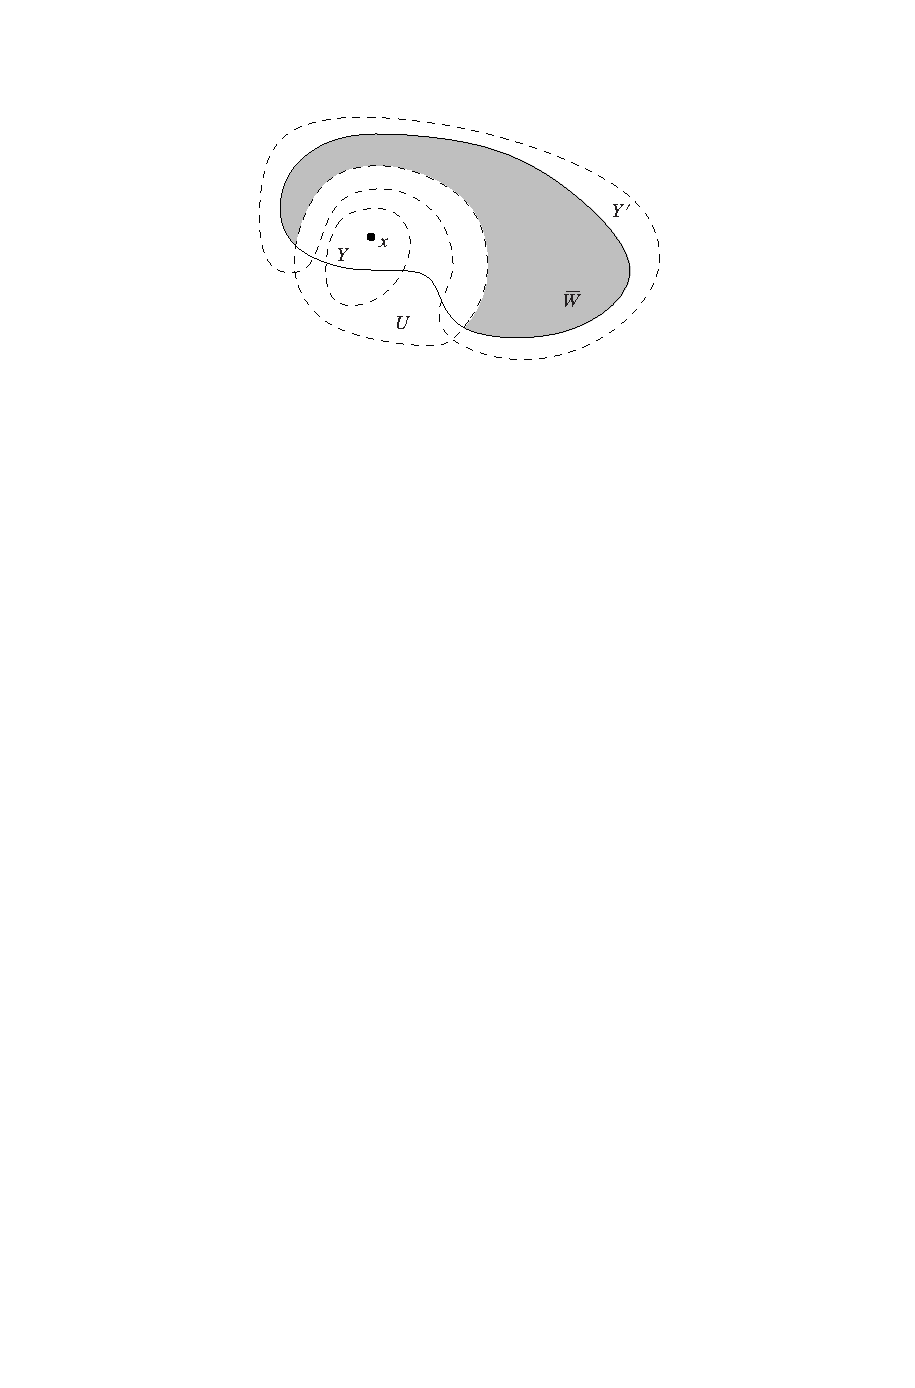
\includegraphics{local-compact}
\end{figure}
\begin{proof}
Suppose $U$ is a neighborhood of $x$. By Proposition~\ref{Hausdorff local compact iff} there is a precompact neighborhood $W$ of $x$. Then $\widebar{W}-U$ is closed in $\widebar{W}$ and therefore compact. Because compact subsets can be separated by open subsets in a Hausdorff space, there are disjoint open subsets $Y$ containing $x$ and $Y'$ containing $\widebar{W}-U$. Let $V=Y-W$. Because $\widebar{V}\sub\widebar{W}$, it is compact.\par
Because $V\sub Y\sub X-Y'$, we have $\widebar{V}\sub\widebar{Y}\sub X-Y'$, and thus $\widebar{V}\sub\widebar{W}-Y'$. Now the fact $\widebar{W}-U\sub Y'$ means $\widebar{W}-Y'\sub U$, thus $\widebar{V}\sub U$.
\end{proof}
\begin{proposition}
Any open or closed subset of a locally compact Hausdorff space is a locally compact Hausdorff space.
\end{proposition}
\begin{theorem}[\textbf{Baire Category Theorem}]
In a locally compact Hausdorff space or a complete metric space, every countable collection of dense open subsets has a dense intersection.
\end{theorem}
\begin{proof}
Let $X$ be a space satisfying either of the hypotheses, and suppose $\{V_n:n\in\N\}$ is a countable collection of dense open subsets of $X$. To show that $\{V_n\}$ is dense, it suffices to show that every nonempty open subset of $X$ containsat least one point of the intersection. Let $U\sub X$ be an arbitrary nonempty open subset.\par
First consider the case in which $X$ is a locally compact Hausdorff space. Since
$V_1$ is dense, $U\cap V_1$ is nonempty, so by Lemma~\ref{local compact precompact} there is a nonempty precompact open subset $W_1$ such that $\widebar{W}_1\sub U\cap V_1$. Similarly, there is a nonempty precompact open subset $W_2$ such that $\widebar{W}_2\sub W_1\cap V_2\sub U\cap V_1\cap V_2$. Continuing by induction, we obtain a sequence of nested nonempty compact sets 
\[\widebar{W}_1\sups\widebar{W}_2\sups\cdots\sups\widebar{W}_n\sups\cdots\] 
such that $\widebar{W}_1\sub U\cap V_1\cap\cdots\cap V_n$. Since $W_1$ is compact, there is a point $x\in\bigcap_{n}W_n$ which is clearly in $U$ and also in $\bigcap_{n}V_n$.\par
In the case that $X$ is a complete metric space, we modify the above proof as
follows. At the inductive step, since $W_{n-1}\cap V_n$ is open and nonempty, there is some
point $x_n$ and positive number $\varepsilon_n$ such that $\B(x_n,\varepsilon_n)\sub W_{n-1}\cap V_n$. Choosing $r_n< \min\{\varepsilon_n,1/n\}$, we obtain a sequence of nested closed balls such that $\widebar{\B}(x_n,r_n)\sub U\cap V_1\cap \cdots\cap V_n$. Because $r_n\to 0$, the centers $(x_n)$ form a Cauchy sequence, which converges to a point $x\in U\cap(\bigcap_n V_n)$.
\end{proof}
A topological space with the property that every countable union of dense open subsets is dense is called a \textbf{Baire space}. Thus the Baire category theorem is simply the statement that locally compact Hausdorff spaces and complete metric spaces are Baire spaces. Since the property of being a Baire space is a topological one, any space that is homeomorphic to a complete metric space is also a Baire space.\par
The Baire category theorem has a useful complementary reformulation. A subset $F$ of a topological space $X$ is said to be \textbf{nowhere dense} if $\widebar{F}$ has dense complement, and $F$ is said to be \textbf{meager} if it can be expressed as a union of countably many nowhere dense subsets.
\begin{proposition}
In a Baire space, every meager subset has dense complement.
\end{proposition}
\begin{corollary}\label{countable closed isolated}
In a locally compact Hausdorff space or a complete metric space, every nonempty countable closed subset contains at least one isolated point.
\end{corollary}
\begin{proof}
Assume $X$ is such a space. Let $A\sub X$ be a nonempty countable closed subset, and assume that $A$ has no isolated points. The fact that $A$ is closed in $X$ means that $A$ itself is either a locally compact Hausdorff space or a complete metric space. For each $a\in A$, the singleton $\{a\}$ is nowhere dense in $A$: it is closed in $A$ because $A$ is Hausdorff, and it contains no nonempty open subset because $A$ has no isolated points. Since $A$ is a countable union of singletons, the Baire category theorem implies that $A$ has empty interior in $A$, which is a contradiction.
\end{proof}
\begin{proposition}
Suppose $q:X\to Y$ is a quotient map and $K$ is a locally compact Hausdorff space. Then the product map $q\times id_K:X\times K\to Y\times K$ is a quotient map.
\end{proposition}
\begin{proof}
We need to show that $q\times id_K$ takes saturated open subsets of $X\times K$ to open
subsets of $Y\times K$. Let $U\sub X\times K$ be a saturated open subset. Given $(x_0,k_0)\in U$,we will show that $(x_0,k_0)$ has a saturated product neighborhood $W\times J$ contained in $U$. It then follows that $q(W)\times J$ contains $\big(q(x_0),k_0\big)$, is contained in $(q\times id_K)(U)$, and is open (since $q(W)$ is the image of a saturated open subset under the quotient map $q)$. Thus $(q\times id_K)(U)$ is open in $Y\times K$. Now we proceed to prove the existence of the desired saturated product neighborhood.\par
For any subset $W\sub X$, we define its saturation to be $\mathrm{Sat}(W)=q^{-1}(q(W))$. It is the smallest saturated subset of $X$ containing $W$.\par
By definition of the product topology, $(x_0,k_0)$ has a product neighborhood $W_0\times J_0\sub U$. By Lemma~\ref{local compact precompact}, there is a precompact neighborhood $J$ of $k_0$ such that $\widebar{J}\sub J_0$, and thus $(x_0,k_0)\in W_0\times J_0\sub U$. Because $U$ is saturated, it follows that $\mathrm{Sat}(W_0)\times \widebar{J}\sub U$. Now, $\mathrm{Sat}(W_0)\times J$ is a saturated subset of $X\times K$, but not necessarily open (since $q$ may not be an open map). We will show that there exists an open subset $W_1\sub X$ containin $\mathrm{Sat}(W_0)$ such that $W_1\times \widebar{J}\sub U$. To prove this, fix some $x\in \mathrm{Sat}(W_0)$. For any $k\in \widebar{J}$, $(x,k)$ has a product neighborhood in $U$. Finitely many of these cover the compact set $\{x\}\times\widebar{J}$, call them $V_1\times J_1,\dots,V_m\times J_m$. If we set $V_x=V1\cap\cdots\cap V_m$, then $V_x$ is a neighborhood
of $\{x\}$ such that $V_x\times\widebar{J}\sub U$. Taking $W_1$ to be the union of all such sets $V_x$ for $x\in\mathrm{Sat}(W_0)$ proves the claim.\par
Repeating this construction, we obtain a sequence of open subsets $W_i\sub X$ such
that
\[W_0\sub\mathrm{Sat}(W_0)\sub W_1\sub\mathrm{Sat}(W_1)\cdots\]
and $W_i\times\widebar{J}\sub U$. Let $W$ be the union of all the $W_i$'s. Then $W$ is open because it is a union of open subsets, and $W\times J\sub U$. Moreover, $W\times J$ is saturated: if $(x,k')\in W\times J$, then $x$ is in some $W_i$, and if $(x',k)$ is any point in the same fiber, then $x'\in W_{i+1}$, so $(x',k)\in W\times J$ as well. Thus $W\times J$ is the required saturated product neighborhood of $(x_0,k_0)$.
\end{proof}
\begin{exercise}
Finite intersections of open dense subsets of $M$ are open and dense in $M$, where $M$ is a metric space.
\end{exercise}
\begin{exercise}\label{open dense intersection}
Let $D_k,k\in\N$, be open dense subsets of $\K^n$ and $D:=\bigcap_kD_k$. Show the following:
\begin{itemize}
\item[$(\rmnum{1})$]$D$ is dense in $\K^n$.
\item[$(\rmnum{2})$]$D$ is uncountable.
\end{itemize}
And it follows that no countable dense subset of $\K^n$ can be obtained as the intersection of a countable family of open sets.
\end{exercise}
\begin{proof}
$(\rmnum{1})$ Directly coms from Baire category theorem. For $(\rmnum{2})$, assume that $D$ is countable, say $D=\{x_m\in\K^n:m\in\N\}$, so $D=\bigcup_m\{x_m\}$. Since every $\{x_m\}^c$ is dense in $\K^n$, again from the Baire category theorem we know that $\bigcap_k\{x_m\}^c\cap\bigcap_{k}D_k$ is dense in $\K^n$. But 
\[D^c\cap D=\big(\bigcup_m\{x_m\}\big)^c\cap\bigcap_{k}D_k=\bigcap_k\{x_m\}^c\cap\bigcap_{k}D_k=\emp\]
which is a contradiction.
\end{proof}
\begin{exercise}
Show that there is no function from $\R$ to $\R$ which is continuous at each rational point
and discontinuous at each irrational point.
\end{exercise}
\begin{proof}
Let $f$ be a such function. Consider $D_k:=\{x\in\R:\omega_f(x)<1/k\}$ for all $k\in\N^{\times}$, where $\omega_f$ is the modulus of continuity. By definition $D_k$ is open. But then $\Q\sub D_k$ and $\bigcap_{k}D_k=\Q$, contradicting Exercise~\ref{open dense intersection}.
\end{proof}
\section{Final topologies and Quotient spaces}
\subsection{Final topology}
\begin{definition}
Let $(X_\alpha)$ be a family of topological spaces and $f_\alpha:X_\alpha\to Y$ be a family of maps. A topology $\mathcal{T}$ on $Y$ is said to be 
\textbf{final with respect to the functions $\bm{(f_\alpha)}$} if, for any topological space $Z$ and function $g:Y\to Z$, $g$ is continuous if and only if $g\circ f_\alpha:X_\alpha\to Z$ 
is continuous for each $\alpha$.
\end{definition}
We shall show that a final topology always exists, but we first point out some simple consequences.
\begin{proposition}\label{final topo prop}
If $\mathcal{T}$ is the final topology on $Y$ with respect to a family of maps $(f_\alpha)$, then
\begin{itemize}
\item[$(a)$] each $f_\alpha:X_\alpha\to Y_\mathcal{T}$ is continuous.
\item[$(b)$] if $\mathcal{T}'$ is any topology on $Y$ such that each $f_\alpha:X_\alpha\to Y_{\mathcal{T}'}$ is continuous, then $\mathcal{T}$ is finer than 
$\mathcal{T}'$.
\end{itemize}
\end{proposition}
The topologies on $Y$ such that each $f_\alpha:X_\alpha\to Y_{\mathcal{T}}$ is continuous forms a category whose morphisms are inclusions. Then by $(b)$ we see that 
the final topology $\mathcal{T}$ is the final object in this category. This justifies the name "final topology".
\begin{proof}
The identity $\id:Y_\mathcal{T}\to Y_\mathcal{T}$ is continuous and hence $\id\circ f_\alpha:X_\alpha\to Y_{\mathcal{T}}$ is continuous for each $\alpha$ in $A$. Since 
$\id\circ f_\alpha=f_\alpha$, it follows that $f_\alpha$ is continuous.\par
Let $g:Y_{\mathcal{T}}\to Y_{\mathcal{T}'}$ be the identity function. Then $g\circ f_\alpha=f_\alpha:X_\alpha\to Y_{\mathcal{T}'}$ is continuous for each $\alpha$ in $A$. 
Hence $g$ is continuous, and so $\mathcal{T}$ is finer than $\mathcal{T}'$.
\end{proof}
We now show that the final topology exists. We suppose given $(X_\alpha)$ and $(f_\alpha)$ as before.
\begin{proposition}
The final topology $\mathcal{T}$ on $Y$ with respect to $(f_\alpha)$ exists and is characterised by the following conditions:
\begin{equation}\label{final topo char-1}
\text{If $U\sub Y$, then $U$ is open in $\mathcal{T}$ if and only if $f_\alpha^{-1}(U)$ is open in $X_\alpha$ for each $\alpha$ in $A$}.
\end{equation}
\end{proposition}
\begin{proof}
First we show that the given condition $(\ref{final topo char-1})$ does define a topology. Clearly $\emp$, $Y$ are open in $\mathcal{T}$. If $U$, $V$ are open in 
$\mathcal{T}$, then
\[f_\alpha^{-1}(U\cap V)=f_\alpha^{-1}(U)\cap f^{-1}_\alpha(V)\]
which is open in $X_\alpha$, and so $U\cap V$ belongs to $\mathcal{T}$. Similarly, the formula $f_\alpha^{-1}(\bigcup_iU_i)=\bigcup_if_\alpha^{-1}(U_i)$ shows that the 
union of any family of sets open in $\mathcal{T}$ is again open in $\mathcal{T}$. Therefore $(\ref{final topo char-1})$ does define a topology.\par
We now prove that this topology is the final topology. Clearly, each $f_\alpha:X_\alpha\to Y_{\mathcal{T}}$ is continuous. Suppose $g:Y_{\mathcal{T}}\to Z$ is a function 
where $Z$ is a topological space. If $g$ is continuous, then so is each composite $g\circ f_\alpha$. Suppose, conversely, that each $g\circ f_\alpha$ is continuous. Let 
$U$ be open in $Z$. Then
\[(g\circ f_\alpha)^{-1}(U)=f_\alpha^{-1}(g^{-1}(U))\]
and, therefore, $f^{-1}_\alpha(g^{-1}(U))$ is open in $X_\alpha$. It follows that $g^{-1}(U)$ is open in $Y_\mathcal{T}$. Hence $g$ is continuous, as we were required 
to prove.
\end{proof}
\begin{example}
Let $X=\coprod_\alpha X_\alpha$ be the disjoint union of the underlying sets of the family $(X_\alpha)_{\alpha\in A}$ of topological spaces, and let $i_\alpha:X_\alpha\to X$ 
be the injections. The final topology on $X$ with respect to $(i_\alpha)$ is called the disjoint union topology.
\end{example}
By means of the topological disjoint union we can reduce final topologies with respect to a family $(f_\alpha)$ to final topologies with respect to a single function $f$.
\begin{proposition}
Let $X$ be the sum of spaces $(X_\alpha)$ and let $f:X\to Y$ be the function determined by $(f_\alpha)$. Then the final topologies on $Y$ with respect to $f$ and with 
respect to $(f_\alpha)$ coincide.
\end{proposition}
\begin{proof}
Let $i_\alpha:X_\alpha\to X$ be the injection. Let $g:Y\to Z$ be a function where $Z$ is a topological space. Then
\[g\circ f_\alpha=g\circ f\circ i_\alpha.\]
Therefore $g\circ f$ is continuous if and only if each $g\circ f\circ i_\alpha$ is continuous. Thus the conditions $g$ is continuous if and only if $g\circ f$ is 
continuous, and $g$ is continuous if and only if each $g\circ f_\alpha$ is continuous, are equivalent.
\end{proof}
\subsection{Quotient maps}
Let $X$ be a topological space, $Y$ be any set, and $q:X\to Y$ be a surjective map. The final topology with respect to the map $q$ is called the \textbf{quotient topology} induced by the map $q$. 
If $X$ and $Y$ are topological spaces, a map $q:X\to Y$ is called a \textbf{quotient map} if it is surjective and $Y$ has the quotient topology induced by $q$. Once $q$ is known to be surjective, to say it is a quotient map is the same as saying that $V$ is open in $Y$ if and only if $q^{-1}(V)$ is open in $X$. It is immediate from the definition that every quotient map is continuous.\par
\begin{proposition}[\textbf{Properties of Quotient Maps}]
\mbox{}
\begin{itemize}
\item[$(a)$]Any composition of quotient maps is a quotient map.
\item[$(b)$]An injective quotient map is a homeomorphism.
\item[$(c)$]If $q:X\to Y$ is a quotient map, a subset $K\sub Y$ is closed if and only if $q^{-1}(K)$ is closed in $X$.
\item[$(d)$]If $q:X\to Y$ is a quotient map and $U\sub X$ is a saturated open or closed subset,
then the restriction $q|_{U}:U\to q(U)$ is a quotient map.
\item[$(e)$]If $\{q_\alpha:X_\alpha\to Y_\alpha\}_{\alpha\in A}$ is an indexed family of quotient maps, then the map $q:\coprod_{\alpha\in A}X_\alpha\to\coprod_{\alpha\in A}Y_\alpha$ whose restriction to each $X_\alpha$ is equal to $q_{\alpha}$ is a quotient map.
\end{itemize}
\end{proposition}
\begin{proposition}\label{quotient second countable}
Suppose $P$ is a second countable space and $M$ is a quotient space of $P$. If $M$ is locally Euclidean, then it is second countable. Thus if $M$ is locally Euclidean and Hausdorff, it is a manifold.
\end{proposition}
\begin{proof}
Let $q:P\to M$ denote the quotient map, and let $\mathcal{U}$ be a cover of $M$ by
coordinate balls. The collection $q^{-1}(\mathcal{U})=\{q^{-1}(U):U\in\mathcal{U}\}$
is an open cover of $P$, which has a countable subcover since $P$ is Lindel\"of. If we let $\mathcal{U}'\sub\mathcal{U}$ denote a countable subset of $\mathcal{U}$ such that $q^{-1}(\mathcal{U}')$ covers $P$, then $\mathcal{U}'$ is a countable cover of $M$ by coordinate balls. Each such ball is second countable, so $M$ is also second countable.
\end{proof}
The following result gives a useful class of quotient maps.
\begin{proposition}
Let $f:X\to Y$ be a continuous surjection. If $f$ is an open map, or a closed map, then $f$ is an quotient map.
\end{proposition}
\begin{proof}
Suppose that $f$ is an open map. Let $U$ be a subset of $Y$. By continuity, if $U$ is open in $Y$ then $f^{-1}(U)$ is open in $X$. On the other hand $f$ is a surjection, 
so $f(f^{-1}(U))=U$. Hence $f^{-1}(U)$ is open if and only if $U$ is open. A similar proof applies with open replaced by closed.
\end{proof}
\begin{corollary}
A continuous surjection from a compact space to a Hausdorff space is an quotient map.
\end{corollary}
\begin{proof}
Such a map is closed.
\end{proof}
\subsection{Hausdorff condition of quotient spaces}
Typically, to prove that a given quotient space is Hausdorff, one has to resort to the definition. For open quotient maps, however, we have the following criterion
\begin{proposition}\label{quotient Hausdorff}
Suppose $q:X\to Y$ is an open quotient map. Then $Y$ is Hausdorff if and only if the set $\mathcal{R}:=\{(x_1,x_2):q(x_1)=q(x_2)\}$ is closed in $X\times X$.
\end{proposition}
\begin{proof}
First assume $Y$ is Hausdorff. If $(x_1,x_2)\notin\mathcal{R}$, then there are disjoint neighborhoods $V_1$ of $q(x_1)$ and $V_2$ of $q(x_2)$, and it follows that $q^{-1}(V_1)\times q^{-1}(V_2)$ is a neighborhood of $(x_1,x_2)$ that is disjoint from $\mathcal{R}$. Thus $\mathcal{R}$ is closed. (This implication does not require the assumption that $q$ is open.)\par
Conversely, assume $\mathcal{R}$ is closed. Given distinct points $y_1,y_2\in Y$, choose $x_1,x_2\in X$ such that $q(x_i)=y_i$. Because $(x_1,x_2)\notin\mathcal{R}$, there is a product neighborhood $U_1\times U_2$ of $(x_1,x_2)$ in $X\times X$ that is disjoint from $\mathcal{R}$. Since $q$ is open, $q(U_1)$ and $q(U_2)$ are disjoint neighborhoods of $y_1$ and $y_2$, respectively.
\end{proof}
\begin{corollary}
Suppose $\sim$ is an equivalence relation on a space $X$. If the quotient map $X\to X/$$\sim$ is an open map, then $X/$$\sim$ is Hausdorff if and only if $\sim$ is a closed subset of $X\times X$.
\end{corollary}
\begin{theorem}
Suppose $X$ is a compact Hausdorff space and $q:X\to Y$ is a quotient map. Then the following are equivalent.
\begin{itemize}
\item[$(a)$]$Y$ is Hausdorff.
\item[$(b)$]$q$ is a closed map.
\item[$(c)$]The set $\mathcal{R}=\{(x_1,x_2):q(x_1)=q(x_2)\}$ is closed in $X\times X$.
\end{itemize}
\end{theorem}
\begin{proof}
The implicaton $(a)\Rightarrow(b)$ is immediate by closed map lemma, and $(a)\Rightarrow(c)$ is proved just as in Proposition~\ref{quotient Hausdorff}.\par
Next we prove $(b)\Rightarrow(a)$. Assuming $q$ is a closed map, we begin by showing that its fibers are compact. Every point $y\in Y$ is the image of some $x\in X$, and since $\{x\}$ is a closed subset of $X$, it follows that $\{y\}=q(\{x\})$ is a closed subset of $Y$. Thus by continuity, the fiber $q^{-1}(\{y\})$ is closed in $X$ and hence compact.\par 
To prove that $Y$ is Hausdorff, suppose $y_1$ and $y_2$ are distinct points of $Y$. Then we can prove the disjoint compact subsets $q^{-1}(y_1)$ and $q^{-1}(y_2)$ of $X$ have disjoint neighborhoods $U_1$ and $U_2$, respectively. Define subsets $W_1,W_2\sub Y$ by
\[W_i=Y-q(X-U_i)=\{y\in Y:q^{-1}(y)\sub U_i\}\]
Then $y_i\in W_i$ for each $i$ by construction, and $W_1$ and $W_2$ are disjoint because $U_1$ and $U_2$ are. To complete the proof, the fact that $q$ is closed implies that $W_i$ is open.\par
Finally, we prove $(c)\Rightarrow(a)$. Assuming that $\mathcal{R}$ is closed, we start again by showing that $q$ has compact fibers. Given $y\in Y$ and $x\notin q^{-1}(y)$, let $x_1$ be any point in $q^{-1}(y)$. (Such a point exists because $q$ is surjective.) Because $\mathcal{R}$ is closed and $(x,x_1)\notin\mathcal{R}$, there is a product neighborhood $U_1\times U_2$ of $(x_1,x)$ that is disjoint from $\mathcal{R}$. It follows that $U_2$ is a neighborhood of $x$ disjoint from $q^{-1}(y)$, for if $x_2$ were a point in $U_2\cap q^{-1}(y)$, then $(x_1,x_2)$ would lie in $\mathcal{R}\cap(U_1\times U_2)$, which is empty. Thus $q^{-1}(y)$ is closed in $X$ and hence compact.\par
Now let $y_1$ and $y_2$ be distinct points in $Y$. As before, there are disjoint open
subsets $U_1\sups q^{-1}(y_1)$ and $U_2\sups q^{-1}(y_2)$, and we define $W_1,W_2$ as before. These are disjoint sets containing $y_1$ and $y_2$, respectively, so we need only show they are open. Because $q$ is a quotient map, $W_i$ is open if and only if $q^{-1}(W_i)$ is open, which is the case if and only if $X-q^{-1}(W_i)$ is closed. From the definition of $W_i$, it follows that
\begin{align*}
X-q^{-1}(W_i)&=\{x\in X:q(x)\notin W_i\}=\{x\in X:q^{-1}(q(x))\nsubseteq U_i\}\\
&=\{x\in X:\exists x\in X-U_i\quad\text{s.t.}\quad q(x)=q(x')\}\\
&=\pi_1(\mathcal{R}\cap(X\times X-U_i))
\end{align*}
where $\pi_1:X\times X\to X$ is the projection on the first factor. Observe that $\pi_1$ is a closed map by the closed map lemma. Our hypothesis on $\mathcal{R}$ implies that $\mathcal{R}\cap(X\times X-U_i)$ is closed in $X\times X$, and therefore $X-q^{-1}(W_i)$ is closed in $X$.
\end{proof}
\subsection{Recognizing Quotient Maps Between Known Spaces}
Suppose $q:X\to Y$ is a map. A subset $U\sub X$ is said to be \textbf{saturated} with respect to $q$ if $U=q^{-1}(V)$ for some subset $V\sub Y$, that is, $q^{-1}(q(U))=U$. Equivalently, $U$ is a union of fibers.
\begin{proposition}\label{quotient map iff}
A continuous surjective map $q:X\to Y$ is a quotient map if and only if it takes saturated open subsets to open subsets, or saturated closed subsets to closed subsets.
\end{proposition}
\begin{proof}
If $q$ is a quotient map and $U$ is a saturated open subsets. Then since $U=q^{-1}(q(U))$ is open, we know $q(U)$ is open.\par
Conversely, if $q$ takes saturated open subsets to open subsets. Let $V\sub Y$ be such that $q^{-1}(V)$ is open in $X$, then since $q(q^{-1}(V))=V$, we know $q^{-1}(V)$ is saturated. Hence by our assumption $V=q(q^{-1}(V))$ is open.
\end{proof}
\begin{proposition}\label{quotient open closed}
If $q:X\to Y$ is a surjective continuous map that is also an open or closed map, then it is a quotient map.
\end{proposition}
\begin{proof}
If $q$ is open, it takes saturated open subsets to open subsets (because it takes
all open subsets to open subsets). If $q$ is closed, it takes saturated closed subsets to closed subsets. In either case, it is a quotient map by Proposition~\ref{quotient map iff}.
\end{proof}
\begin{proposition}\label{closed open map inj surj bij}
Suppose $X$ and $Y$ are topological spaces, and $f:X\to Y$ is a continuous map that is either open or closed.
\begin{itemize}
\item[$(a)$]If $f$ is injective, it is a topological embedding.
\item[$(b)$]If $f$ is surjective, it is a quotient map.
\item[$(c)$]If $f$ is bijective, it is a homeomorphism.
\end{itemize}
\end{proposition}
\subsection{Subspaces, products, and quotient maps}
\subsubsection{Subspaces of a quotient space}
The following result is important in itself and will also help the discussion of examples of quotient spaces.
Let $f:X\to Y$ be an quotient map, and let $A\sub X$. Then $A$, $f(A)$ are subspaces of $X$, $Y$ respectively, and we ask: is $g=f|_A$ an quotient
map?
\begin{theorem}\label{quotient restriction iff}
The following conditions are equivalent.
\begin{itemize}
\item[$(a)$] $g=f|_A:A\to f(A)$ is an quotient map,
\item[$(b)$] each $g$-saturated set which is open in $A$ is the intersection of $A$ with an $f$-saturated set open in $X$.
\end{itemize}
\end{theorem}
\begin{proof}
We state an elementary result in set theory: if $V\sub f(A)$ and $V'\sub Y$, then
\[V=f(A)\cap V'\iff g^{-1}(V)=A\cap f^{-1}(V').\]
For $(a)\Rightarrow(b)$, let $U$ be open in $A$ and $g$-saturated. Then by Proposition~\ref{quotient map iff} $V=g(U)$ is open in $f(A)$, whence $V=f(A)\cap V'$ where 
$V'$ is open in $Y$. So
\[U=g^{-1}(g(U))=g^{-1}(f(A)\cap V')=A\cap f^{-1}(V').\]
Clearly, $f^{-1}(V')$ is open in $X$ and $f$-saturated.\par
For $(b)\Rightarrow(a)$, let $V$ be a subset of $f(A)$ such that $g^{-1}(V)$ is open in $A$. Since $g^{-1}(V)$ is $g$-saturated, by condition $(b)$ we have 
$g^{-1}(V)=A\cap U$ for some $f$-saturated set $U$ open in $X$. Note that $U=f^{-1}(f(U))$, so we can write
\[g^{-1}(V)=A\cap f^{-1}(f(U)),\]
and therefore $V=f(A)\cap f(U)$. Then $V$ is open in $f(A)$, which implies $g$ is a quotient map.
\end{proof}
\begin{corollary}\label{quotient restriction on saturated open}
Each of the following conditions implies that $g=f|_A$ is an quotient map.
\begin{itemize}
\item[$(a)$] For all $U$, if $U$ is $g$-saturated and open (closed, respectively) in $A$, then $f^{-1}(f(U))$ is open (closed, respectively) in $X$.
\item[$(b)$] The set $A$ is $f$-saturated and open (closed) in $X$. 
\end{itemize}
\end{corollary}
\begin{proof}
For any subset $U$ of $A$, we have
\[g^{-1}(g(U))=A\cap f^{-1}(f(U)).\]
Moreover, $f^{-1}(f(U))$ is an $f$-saturated set in $X$. So if $(a)$ holds, then condition $(b)$ of Theorem~\ref{quotient restriction iff} is satisfied.\par
We now reduce $(b)$ to $(a)$. Let $U$ be $g$-saturated and open in $A$. Then 
\[f^{-1}(f(U))\sub f^{-1}(f(A))=A,\]
whence
\[f^{-1}(f(U))=g^{-1}(g(U))=U.\]
Also $U$ is open in $X$ since $A$ is open in $X$.
\end{proof}
\subsubsection{Products of quotient maps}
Let $f:X\to Y$, $f':X'\to Y'$ be quotient maps. It is not true in general that $f\times f':X\times X'\to Y\times Y'$ is an quotient map---an example is 
given below. However we can prove:
\begin{theorem}\label{quotient product}
Let $f:X\to Y$ be an quotient map and let $B$ be a locally compact. Then
\[f\times\id:X\times B\to Y\times B\]
is an quotient map.
\end{theorem}
\begin{proof}
Let $W\sub X\times B$ be open and saturated with respect to $h:=f\times\id$. We must prove that $h(W)$ is open in $Y\times B$. To this end, let $(y_0,b_0)\in h(W)$ and 
suppose $y_0=f(x_0)$. Then $(x_0,b_0)\in W$ since $W$ is saturated. Let $B_0$ be the subset of $B$ such that
\[\{x_0\}\times B_0=(\{x_0\}\times B)\cap W;\]
this is the "$x_0$-section" of $W$. Since $W$ is open, $B_0$ is a neighbourhood of $b_0$. Since $B$ is locally compact, by Theorem~\ref{Hausdorff local compact iff} 
$B_0$ contains a precompact neighbourhood $C$ of $b_0$.
\begin{figure}[htbp]
\centering
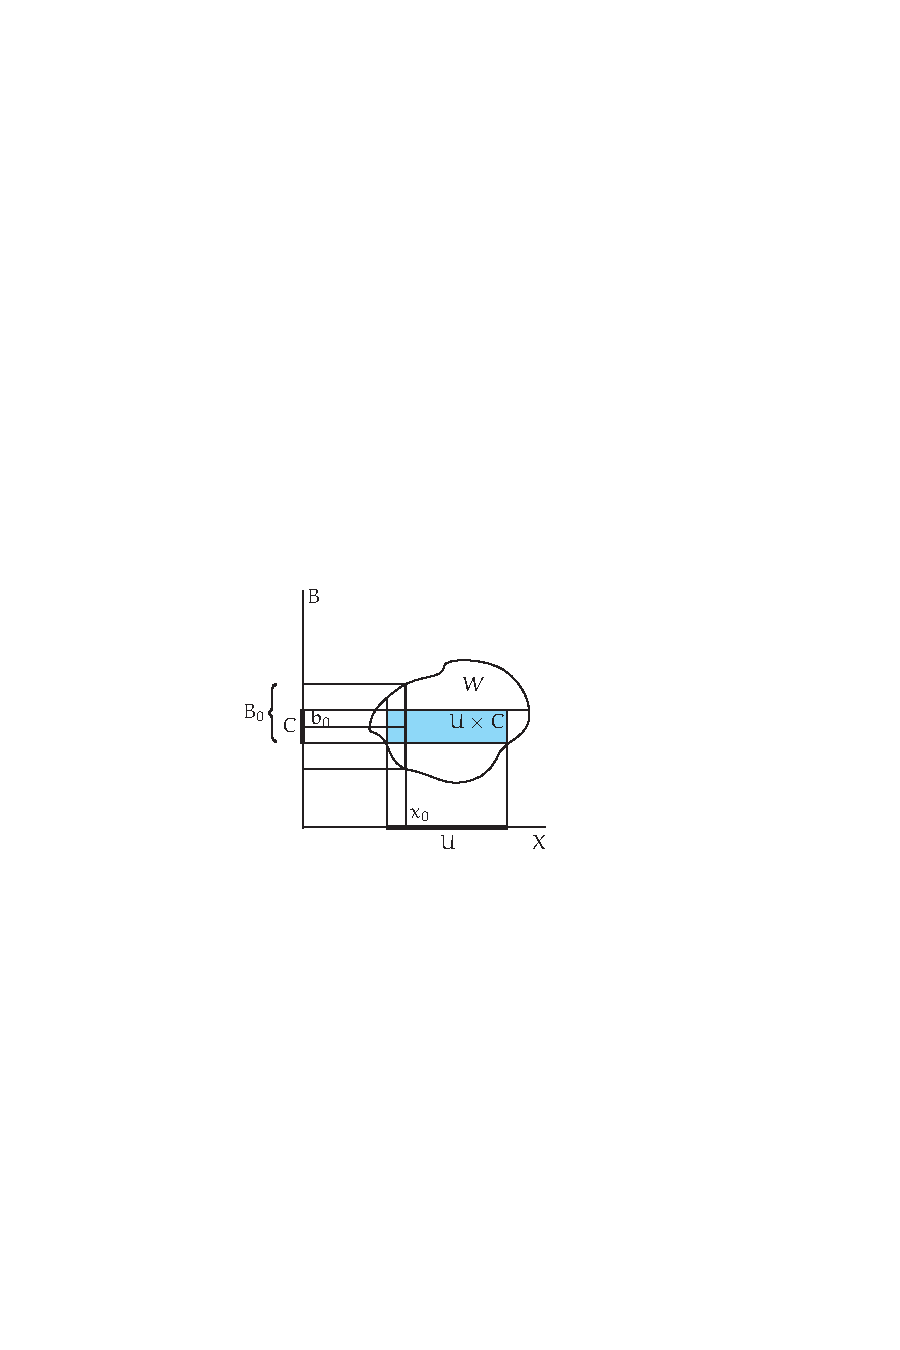
\includegraphics{quotient-product}
\end{figure}

Let $U\sub X$ be the largest set such that $U\times\widebar{C}\sub W$, that is,
\[U=\{x\in X:\{x\}\times\widebar{C}\sub W\}.\]
Then
\[(y_0,b_0)\in f(U)\times\widebar{C}\sub h(W).\]
So to prove that $h(W)$ is a neighbourhood of $(y_0,b_0)$, it is sufficient to prove that $f(U)$ is a neighbourhood of $y_0$.\par
Let $x\in U$ so that $\{x\}\times\widebar{C}\sub W$. Since $\widebar{C}$ is compact and $W$ is open, there is a neighbourhood $V$ of $x$ such that 
$V\times\widebar{C}\sub W$ (tube lemma). This implies that $V\sub U$, by definition of $U$. So $U$ is open.\par
We have $U\sub f^{-1}(f(U))$ and
\[f^{-1}(f(U))\times\widebar{C}=h^{-1}(h(U\times\widebar{C}))\sub h^{-1}(h(W))=W.\]
So $f^{-1}(f(U))\sub U$, by definition of $U$. Hence $U$ is saturated. It follows that $f(U)$ is a neighbourhood of $y_0$.
\end{proof}
\begin{example}
We now show that Theorem~\ref{quotient product} is false without some assumptions on $B$. Let $\pi:\Q\to\Q/\Z$ be the quotient map and let 
$h=\pi\times\id:\Q\times\Q\to(\Q/\Z)\times\Q$. Then $h$ is not an quotient map.\par
Let $r_0=1$ and for each non-zero $n\in\N$ let $r_n=\sqrt{2}/|n|$---thus $r_n$ is irrational and $r_n\to 0$ as $n\to\infty$. Let $A_n$ be any open subset of $[n,n+1]\times\R$
such that the closure of $A_n$ meets $\{n,n+1\}\times\R$ in the two points $(n,r_n)$ and $(n,r_{n+1})$. Let $A$ be the union of these sets $A_n$, $n\in\N$, and let 
$B=\widebar{A}\cap (\Q\times\Q)$. Then $B$ is closed in $\Q\times\Q$ and saturated with respect to $h$. By our construction of $r_n$, we see that in 
$(\Q/\Z)\times\Q$ the point $(\pi(0),0)$ belongs to the closure of $h(B)$, so $h(B)$ is not closed. This then implies that $h$ is not a quotient map.
\begin{figure}[htbp]
\centering
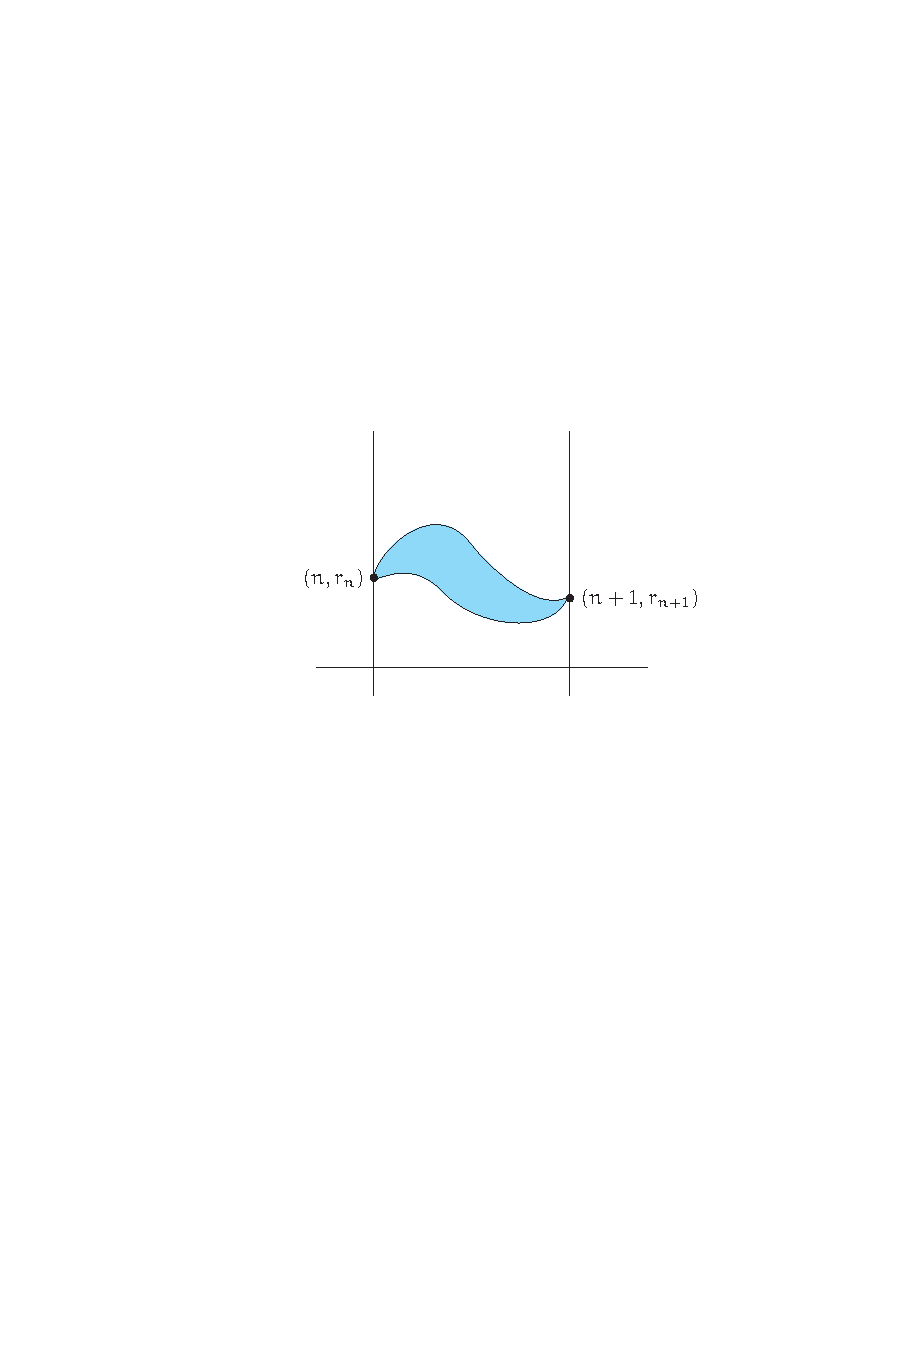
\includegraphics{quotient-product-no}
\caption{The open subset $A_n$.}
\end{figure}
\end{example}
\section{Topological Manifolds}
\subsection{Definition of Manifolds}
A topological space $M$ is said to be \textbf{locally Euclidean} of dimension $n$ if every point of $M$ has a neighborhood in $M$ that is homeomorphic to an open subset of $\mathbb{R}^n$.
\begin{lemma}\label{locally Euclidean lemma}
A topological space $M$ is locally Euclidean of dimension $n$ if and
only if either of the following properties holds:
\begin{itemize}
\item[$(a)$]Every point of $M$ has a neighborhood homeomorphic to an open ball in $\mathbb{R}^n$.
\item[$(b)$]Every point of M has a neighborhood homeomorphic to $\mathbb{R}^n$.
\end{itemize} 
In addition, $\mathbb{R}^n$ is homeomorphic to an open ball in $\mathbb{R}^n$.
\end{lemma}
\begin{proof}
It is immediate that any space with property $(a)$ or $(b)$ is locally Euclidean of dimension $n$. Conversely, suppose $M$ is locally Euclidean of dimension $n$. Because any open ball in $\R^n$ is homeomorphic to $\R^n$ itself, properties $(a)$ and $(b)$ are equivalent, so we need only prove $(a)$.\par
Given a point $p\in M$, let $U$ be a neighborhood of $p$ that admits a homeomorphism $\varphi:U\to V$, where $V$ is an open subset of $\R^n$. The fact that $V$ is open in $\R^n$ means that there is some open ball $B$ around $\varphi(p)$ that is contained in $V$, and then $\varphi^{-1}(B)$ is a neighborhood of $p$ homeomorphic to $B$.
\end{proof}
Suppose $M$ is locally Euclidean of dimension $n$. If $U\sub M$ is an open subset that is homeomorphic to an open subset of $\mathbb{R}^n$, then $U$ is called a \textbf{coordinate domain}, and any homeomorphism $\varphi$ from $U$ to an open subset of $\mathbb{R}^n$ is called a \textbf{coordinate map}. The pair $(U,\varphi)$ is called a \textbf{coordinate chart} (or just a chart) for $M$. A \textbf{coordinate domain} that is homeomorphic to a ball in $\mathbb{R}^n$ is called a \textbf{coordinate ball}. The preceding lemma shows that every point in a locally Euclidean space is contained in a coordinate ball.\par
The definition of locally Euclidean spaces makes sense even when $n=0$. Because $\R^0$ is a single point, Lemma~\ref{locally Euclidean lemma}$(b)$ implies that a space is locally Euclidean of dimension $0$ if and only if each point has a neighborhood homeomorphic to a one-point space, or in other words if and only if the space is discrete.
\begin{definition}[\textbf{topological manifold}]
An $n$-dimensional \textbf{topological manifold} is a second countable Hausdorff space that is locally Euclidean of dimension $n$.
\end{definition}
The most obvious example of an $n$-manifold is $\R^n$ itself. More generally, any open subset of $\R^n$---or in fact of any $n$-manifold---is again an $n$-manifold, as the next proposition shows.
\begin{proposition}
Every open subset of an $n$-manifold is an $n$-manifold.
\end{proposition}
\begin{proof}
Let $M$ be an $n$-manifold, and let $V$ be an open subset of $M$. Any $p\in V$ has a neighborhood (in $M$) that is homeomorphic to an open subset of $\R^n$; the intersection of that neighborhood with $V$ is still open, still homeomorphic to an open subset of $\R^n$, and is contained in $V$, so $V$ is locally Euclidean of dimension $n$. Since any open subset of a Hausdorff space is Hausdorff and any open subset of a second countable space is second countable, we see that $V$ is an $n$-manifold.
\end{proof}
\begin{theorem}
A separable metric space that is locally Euclidean of dimension $n$ is an $n$-manifold. And the converse is also true.
\end{theorem}
\begin{proof}
Every metric space is Hausdorff, and Theorem~\ref{metric space second countable iff} shows that a separable metric space is second countable. For the converse, separability follows from Theorem~\ref{second countable prop}, and metrizability follows from Urysohn metrization theorem.
\end{proof}
\subsection{Manifolds with boundary}
In many cases we will encounter spaces that would be manifolds except that they have a boundary. The following definition deals with this problem.\par
The closed $n$ dimensional upper half-space $\mathbb{H}^n\sub\mathbb{R}^n$ is defined by
\[\mathbb{H}^n:=\{(x_1,\dots,x_n)\in\mathbb{R}^n:x_n\geq0\}\]
\begin{definition}[\textbf{Manifolds with Boundary}]
An $n$-dimensional manifold with boundary is a second countable Hausdorff space in which every point has a neighborhood homeomorphic either to an open subset of $\mathbb{R}^n$, or to an open subset of $\mathbb{H}^n$.
\end{definition}
Note that, despite the terminology, a manifold with boundary is not necessarily a manifold. When it is important to make the distinction, we say $(U,\varphi)$ is an \textbf{interior chart} if $(U,\varphi_0)$ is an open subset of $\mathbb{R}^n$, and a \textbf{boundary chart} if $(U,\varphi)$ is an open subset of $\mathbb{H}^n$ with $\varphi(U)\cap\partial\H^n\neq\emp$.\par
If $M$ is an $n$-manifold with boundary, we define a coordinate chart for $M$ to be a pair $(U,\varphi)$, where $U\sub M$ is open and $\varphi$ is a homeomorphism from $U$ to an open subset of either $\R^n$ or $\H^n$. Just as in the case of manifolds, the set $U$ is called a \textbf{coordinate domain}, and $\varphi$ is called a coordinate map. We use the notation $\partial\H^n$ to denote the boundary of $\H^n$, and $\Int\H^n$ to denote its interior, considering $\H^n$ as a subset of $\R^n$. For $n>0$, this means
\[\partial\H^n=\{(x_1,\dots,x_n):x_n=0\},\quad\Int\H^n=\{(x_1,\dots,x_n):x_n>0\}.\]
When $n=0$, we have $\H^0=\R^0=\{0\}$, so $\Int\H^0=\H^0$ and $\partial\H^0=\emp$. It follows that $0$-dimensional manifolds with boundary are no different from $0$-manifolds.
\begin{example}
The upper half-spaceHn itself is an nmanifold with boundary, with the identity map as a global coordinate map. Similarly, any closed or half-open interval in $\R$ is a $1$-manifold with boundary, for which charts are easy to construct. Another important example is the closed unit ball $\widebar{\B}^n$ with the Euclidean topology. It is not hard to see intuitively that $\widebar{\B}^n$ is an $n$-manifold with boundary
\end{example}
If $M$ is an $n$-manifold with boundary, a point $p\in M$ is called an \textbf{interior point} of $M$ if it is in the domain of an interior chart; and it is called a \textbf{boundary point} of $M$ if it is in the domain of a boundary chart that takes $p$ to $\partial\H^n$. The \textbf{boundary of $\bm{M}$}, denoted by $\partial M$, is the set of all its boundary points, and its \textbf{interior}, denoted by $\Int M$, is the set of all its interior points.\par
Note that these are new meanings for the terms boundary and interior, distinct from their use earlier in reference to subsets of topological spaces. If $M$ is a manifold with boundary, it might have nonempty boundary in this new sense, irrespective of whether it has any boundary points as a subset of some other topological space. Usually the distinction is clear from the context, but if necessary we can always distinguish the two meanings by referring to the \textbf{topological boundary} (for the original meaning) or the \textbf{manifold boundary} (for this new meaning) as appropriate.
\begin{theorem}\label{manifold boundary int open boundary mani}
If $M$ is an $n$-dimensional manifold with boundary, then $\mathrm{Int}M$ is an open subset of $M$, which is itself an $n$-dimensional manifold without boundary. And $\partial M$ is an $(n-1)$-manifold without boundary.
\end{theorem}
There is a subtlety about these definitions that might not be immediately evident. Although the interior and boundary of $M$ are well-defined subsets whose union is $M$, and it might seem intuitively rather obvious that they are disjoint from each other, we have no way of proving at this stage that a point $p\in M$ cannot be simultaneously a boundary point and an interior point, meaning that there is one interior chart whose domain contains $p$, and another boundary chart that sends $p$ to $\partial\H^n$.
After we have developed some more machinery, you will be able to prove the following theorem.
\begin{theorem}[\textbf{Invariance of the Boundary}]\label{invariance boundary}
If $M$ is a manifold with boundary, then a point of $M$ cannot be both a boundary point and an interior point. Thus $\partial M$ and $\mathrm{Int}M$ are disjoint subsets whose union is $M$.
\end{theorem}
\begin{corollary}
If $M$ is a nonempty $n$-dimensional manifold with boundary, then $\partial M$ is closed in $M$, and $M$ is an $n$-manifold if and only if $\partial M=\emp$.
\end{corollary}
\begin{proof}
Because $\Int M$ is an open subset of $M$ by Proposition~\ref{manifold boundary int open boundary mani}, it follows from Theorem~\ref{invariance boundary} that $\partial M=M\setminus\Int M$ is closed. If $M$ is a manifold, then every point is in the domain of an interior chart, so $M=\Int M$, and it follows from Theorem~\ref{invariance boundary} that $\partial M=\emp$. Conversely, if $\partial M=\emp$, then $M=\Int M$, which is a manifold by Proposition~\ref{manifold boundary int open boundary mani}.
\end{proof}
\begin{corollary}
Let $M$ be a smooth manifold with boundary, let $(U,\varphi)$ be a boundary chart
on $M$, and let $p$ be a point in $\partial M\cap U$. Then $\varphi(p)$ is in $\partial\H^n$. Thus, a coordinate map sends boundary points to boundary points.
\end{corollary}
\begin{proof}
If $p$ is a boundary point, then $\varphi(p)$ is also a boundary point in $\H^n$. Thus by Theorem~\ref{invariance boundary} we know $\varphi(p)\in\partial\H^n$.
\end{proof}
More generally, we have the following result.
\begin{theorem}\label{homeomorphism invariance boundary}
If $M$ and $N$ are smooth manifolds with boundary and $F:M\to N$ is a homeomorphism, then $F(\partial M)=\partial N$, hence $F(\Int M)=F(\Int N)$.
\end{theorem}
\begin{proof}
Since $F$ is a homeomorphism, every boundary point of $M$ is mapped to boundary of $N$, and vise versa. Thus we have $F(\partial M)=\partial N$, and since $M$ is the disjoint union of its interior and boundary, we also have $F(\Int M)=\Int N$.
\end{proof}
\begin{example}\label{Graph mani}
If $U\sub\mathbb{R}^n$ is an open subset and $f:U\to\mathbb{R}^k$ is any continuous map, the graph of $f$ is the subset $\Gamma(f)\sub\mathbb{R}^{n+k}$ defined by
\[\Gamma(f):=\{(x,y)\in\mathbb{R}^{n+k}:x\in U\ \text{and}\ y=f(x)\}\]
with the subspace topology inherited from $\mathbb{R}^{n+k}$. Let $\varPhi_f:U\to\mathbb{R}^{n+k}$ be the continuous injective map
\[\varPhi_f(x)=\big(x,f(x)\big)\]
the the restriction to $\Gamma(f)$ of the projection $\pr:\mathbb{R}^{n+k}\to\mathbb{R}^{n}$ is a continuous inverse for $\Phi_f$. Hence $\Gamma(f)$ is homeomorphic to $U$ and is a manifold.
\end{example}
\begin{example}
Define $\mathbb{RP}^n$ to be the set of $1$-dimensional linear subspaces (lines through the origin) in $\mathbb{R}^{n+1}$, and $\mathbb{CP}^n$ be the set of all $1$-dimensional complex subspaces of $\mathbb{C}^{n+1}$, called $n$-dimensional complex projective space. Topologize them as thequotient $(\mathbb{R}^{n+1}\setminus\{0\})/\mathbb{R}^*$ and $(\mathbb{C}^{n+1}\setminus\{0\})/\mathbb{C}^*$. Then $\mathbb{RP}^n$ is an $n$-manifold, $\mathbb{CP}^{n}$ is a $2n$-manifold.
\end{example}
\begin{example}
Let $X$ be the subset $(\mathbb{R}\times\{0\}\cup(\mathbb{R}\times\{1\}\sub\mathbb{R}^2$. Define an equivalence relation on $X$ by declaring $(x,0)\sim(x,1)$ if $x\neq 0$. Show that the quotient space
$X/$$\sim$ is locally Euclidean and second countable, but not Hausdorff. (This space is called the \textbf{line with two origins})
\end{example}
\begin{example}
Consider the product $\mathbb{R}^d\times\mathbb{R}$, where $\mathbb{R}^d$ means $\mathbb{R}$ with discrete topology. This space is Huasdorff and Locally Euclidean, but not second countable.
\end{example}
\section{Adjunction Spaces}
\begin{definition}
Suppose $X$ and $Y$ are topologicalspaces, $A$ is a closed subspace of $Y$ , and $f:A\to X$ is a continuous map. Let $\sim$ bethe equivalence relation on the disjoint union $X\amalg Y$ generated by $a\sim f(a)$ for all $a\in A$, and denote the resulting quotient space by
\[X\cup_{f}Y:=(X\amalg Y)/\text{$\sim$}\]
Any such quotient space is called an \textbf{adjunction space}, and is said to be formed by
attaching $Y$ to $X$ along $f$. The map $f$ is called the attaching map. Note that the
equivalence relation identifies each point $x\in X$ with all of the points (if any) in $f^{-1}(x)\in A$. If $A=\emp$, then $X\cup_{f} Y$ is just the disjoint union space $X\amalg Y$.
\end{definition}
\begin{theorem}\label{adjunction space prop}
Let $X\cup_{f}Y$ be an adjunction space, and let $q:X\amalg Y\to X\cup_{f}Y$ be the associated quotient map.
\begin{itemize}
\item[$(a)$]The restriction of $q$ to $X$ is a topological embedding, whose image set $q(X)$ is a closed subspace of $X\cup_{f}Y$.
\item[$(b)$]The restriction of $q$ to $Y\setminus A$ is a topological embedding, whose image set $q(Y\setminus A)$ is an open subspace of $X\cup_{f}Y$.
\item[$(c)$]$X\cup_{f}Y$ is the disjoint union of $q(X)$ and $q(Y\setminus A)$.
\end{itemize}
\end{theorem}
\begin{proof}
We begin by showing that $q|_X$ is a closed map. Suppose that $B$ is a closed subset of $X$. To show that $q(B)$ is closed in the quotient space, we need to show that $q^{-1}(q(B))$ is closed in $X\amalg Y$, which is equivalent to showing that its intersections with $X$ and $Y$ are closed in $X$ and $Y$, respectively. From the form of the equivalence relation, it follows that $q^{-1}(q(B))\cap X=B$, which is closed in $X$ by assumption; and $q^{-1}(q(B))=f^{-1}(B)$, which is closed in $A$ by the continuity of $f$, and thus is closed in $Y$ because $A$ is closed in $Y$. It follows, in particular, that $q(X)$ is closed in $X\cup_f Y$.\par
Now $q|_X$ is clearly injective because the equivalence relation does not identify any points in $X$ with each other. Because it is also closed, it is a topological embedding by Proposition~\ref{closed open map inj surj bij}. This proves $(a)$.\par
To prove $(b)$, we just note that $Y\setminus A$ is a saturated open subset of $X\amalg Y$, so the restriction $q|_{Y\setminus A}$ is a quotient map by Corollary~\ref{quotient restriction on saturated open}, and since it is bijective it is a homeomorphism. Its image is open in $X\cup_f Y$ by definition of the quotient topology.\par
Finally, part $(c)$ is an easy consequence of the definition of the equivalence relation.
\end{proof}
Because of the preceding proposition, one typically identifies $X$ with $q(X)$ and $Y\setminus A$ with $q(X\setminus A)$, considering each as a subspace of the adjunction space.
\begin{example}[\textbf{Adjunction Spaces}]
\mbox{}
\begin{itemize}
\item[$(a)$] Suppose $X$ and $Y$ are topological spaces with chosen base points $x\in X$ and $y\in Y$. Let $A=\{y\}\sub Y$, and define $f:A\to X$ by $f(y)=x$. Then the adjunction space $X\cup_f Y$ is just the wedge sum $X\wedge Y$.
\item[$(b)$] Let $A=S^1\sub\widebar{\B}^2$, and let $f:A\to\widebar{\B}^2$ be the inclusion map. Then the adjunction space is homeomorphic to $S^2$.
\end{itemize}
\end{example}
Suppose $M$ and $N$ are $n$-dimensional manifolds with nonempty boundaries, such that $\partial M$ and $\partial N$ are homeomorphic. Let $h:\partial N\to \partial M$ be a homeomorphism. Assuming the theorem on the invariance of the boundary, we conclude that $\partial N$ is a closed subset of $N$, so we can define the adjunction space $M\cup_{h}N$ (considering $h$ as a map into $M)$. This space is said to be formed by \textbf{attaching $\bm{M}$ and $\bm{N}$ together along their boundaries}.
\begin{theorem}\label{attach manifold with boundary}
With $M$, $N$, and $h$ as above, $M\cup_h N$ is an $n$-manifold (without boundary). There are topological embeddings $e:M\to M\cup_{h}N$ and $f:N\to M\cup_{h}N$ whose images are closed subsets of $M\cup_{h}N$ satisfying
\[e(M)\cup f(N)=M\cup_{h}N,\quad e(M)\cap f(N)=e(\partial M)=f(\partial N).\]
\end{theorem}
\begin{proof}
First we need to show that $M\cup_h N$ is locally Euclidean of dimension $n$. Let $q:M\amalg N\to M\cup_h N$ denote the quotient map, and write $S=q(\partial M\cup\partial N)$. Note that $\Int M\amalg\Int N$ is a saturated open subset of $M\amalg N$, and therefore $q$ restricts to a quotient map from $\Int M\amalg\Int N$ onto $(M\cup_h N)\setminus S$. Because this restriction is injective, it is a homeomorphism, and thus $(M\cup_hN)\setminus S$ is locally Euclidean of dimension $n$. Thus we need only consider points in $S$.
\begin{figure}[htbp]
\centering
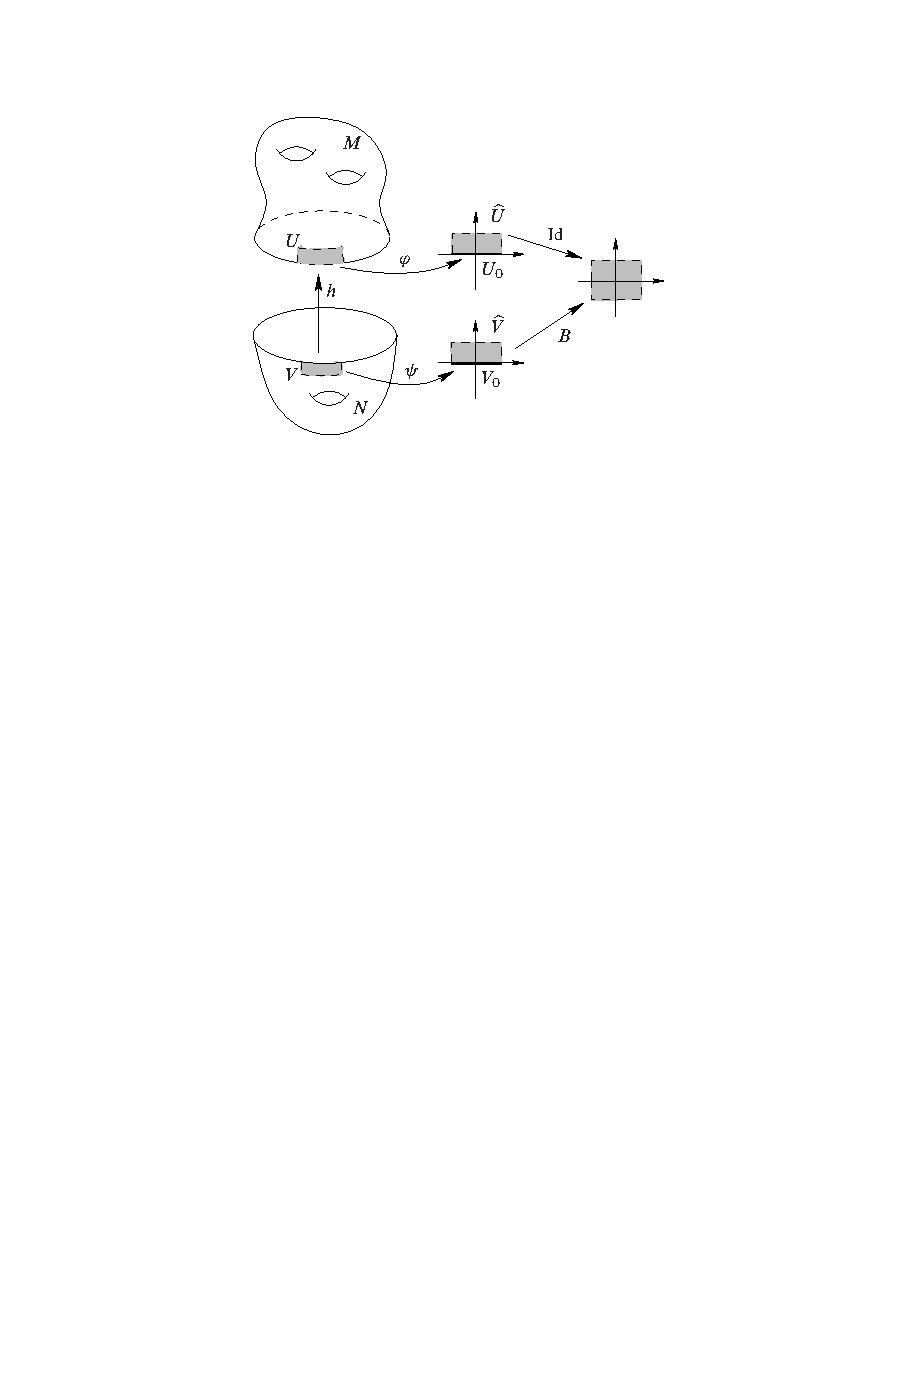
\includegraphics{attach-manifold}
\caption{Attaching along boundaries.}
\end{figure}

Suppose $s\in S$, and let $y\in\partial N$ and $x=h(y)\in\partial M$ be the two points in the fiber $q^{-1}(s)$. We can choose coordinate charts $(U,\varphi)$ for $M$ and $(V,\psi)$ for $N$ such that $x\in U$ and $y\in V$, and let $\widehat{U}=\varphi(U)$, $\widehat{V}=\psi(V)$. It is useful in this proof to identify $\H^n$ with $\R^{n-1}\times[0,+\infty)$ and $\R^n$ with $\R^{n-1}\times\R$. By shrinking $U$ and $V$ if necessary, we may assume that $h(V\cap\partial N)=U\cap\partial M$, and that $\widehat{U}=U_0\times[0,\eps)$ and $\widehat{V}=V_0\times[0,\eps)$ for some $\eps>0$ and some open subsets $U_0,V_0\sub\R^{n-1}$. Then we can write the coordinate maps as 
\[\varphi(x)=(\varphi_0(x),\varphi_1(x)),\quad\psi(y)=(\psi_0(y),\psi_1(y))\]
for some continuous maps $\varphi_0:U\to U_0$, $\varphi_1:U\to[0,\eps)$, $\psi_0:V\to V_0$ and $\psi_1:V\to[0,\eps)$. Our assumption that $x$ and $y$ are boundary points means that $\varphi_1(x)=\psi_1(y)=0$.\par
We wish to assemble these two charts into a map whose image is an open subset of $\R^n$, by matching them up along corresponding points in $\partial M$ and $\partial N$. As they stand, however, the maps $\varphi$ and might not take corresponding boundary points to the same image point, so we need to adjust for that. Both of the restrictions
\[\varphi_0|_{U\cap\partial M}:U\cap\partial M\to U_0,\quad \psi_0|_{V\cap\partial N}:V\cap\partial N\to V_0\]
are homeomorphisms. Define a homeomorphism $\tau:V_0\to U_0$ by
\[\tau=(\varphi_0|_{U\cap\partial M})\circ h\circ(\psi_0|_{V\cap\partial N})^{-1},\]
and let $B:\widehat{V}\to\R^n$ be the map
\[B(x_1,\dots,x_n)=(\tau(x_1,\dots,x_{n-1}),-x_n).\]
Geometrically, $B$ rearranges the boundary points according to the map $\tau$, and then "flips" each vertical line segment above a boundary point to a line segment below the image point. Our construction ensures that for $y\in\partial N$,
\begin{align}\label{attach manifold with boundary-1}
B\circ\psi(y)=(\tau\circ\psi(y),0)=(\varphi_0\circ h(y),0)=\varphi\circ h(y).
\end{align}
Now define $\widetilde{\varPhi}:U\amalg V\to\R^n$ by
\[\widetilde{\varPhi}=\begin{cases}
\varphi(y),&y\in U;\\
B\circ\psi(y),&y\in V.
\end{cases}\]
Because $U\amalg V$ is a saturated open subset of $M\amalg N$, the restriction of $q$ to it is a quotient map onto the neighborhood $q(U\amalg V)$ of $s$, and $(\ref{attach manifold with boundary-1})$ shows that $\widetilde{\varPhi}$ passes
to the quotient and defines an injective continuous map $\varPhi:q(U\amalg V)\to\R^n$. Since $\varphi$, $\psi$, and $B$ are homeomorphisms onto their images, we can define an inverse for $\varPhi$ as follows:
\[\varPhi^{-1}(y)=\begin{cases}
q\circ\varphi^{-1}(y),&y^n\geq 0;\\
q\circ\psi^{-1}\circ B^{-1}(y)&y^n\leq 0.
\end{cases}\]
These two definitions agree where they overlap, so the resulting map is continuous by the gluing lemma. Thus $\varPhi$ is a homeomorphism. Note that the image of $\varPhi$ is exactly $U_0\times(-\eps,\eps)$, which is open in $\R^n$. Therefore $M\cup_hN$ is locally Euclidean of dimension $n$.\par
The quotient space $M\cup_h N$ is second countable by Proposition~\ref{quotient second countable}. To prove that it is Hausdorff, we need to show that the fibers of $q$ can be separated by saturated open subsets. It is straightforward to check on a case-by-case basis that the preimages of sufficiently small coordinate balls will do.\par
It follows immediately from Proposition~\ref{adjunction space prop}$(a)$ that the quotient map $q$ restricts to a topological embedding of $M$ into $M\cup_h N$ with closed image. On the other hand, because $h$ is a homeomorphism, it is easy to see that $M\cup_h N$ is also equal to
$N\cup_{h^{-1}}M$, so $q$ also restricts to a topological embedding of $N$ with closed image. The union of the images of these embeddings is all of $M\cup_hN$, and their intersection is the set $S$ defined above, which is exactly the image of either boundary.
\end{proof}
Here is an important example of the preceding construction.
\begin{example}[\textbf{The Double of a Manifold with Boundary}]
Suppose $M$ is an ndimensional manifold with boundary. If $h:\partial M\to \partial M$ is the identity map, the resulting quotient space $M\cup_{h}M$ is denoted by $D(M)$ and called the \textbf{double of $\bm{M}$}. It can be visualized as the space obtained by attaching two copies of $M$ to each other along their common boundary. (If $\partial M=\emp$, then $D(M)$ is just the disjoint union of two copies of $M)$
\end{example}
The following proposition is an immediate consequence of Theorem~\ref{attach manifold with boundary}.
\begin{proposition}
Every $n$-manifold with boundary is homeomorphic to a closed subset of an $n$-manifold without boundary.
\end{proposition}
This construction can be used to extend many results about manifolds to manifolds with boundary. For example, any property that holds for all closed subsets of manifolds is also shared by manifolds with boundary.
\section{Paracompactness}
Let $X$ be a topological space. A collection $\mathcal{A}$ of subsets of $X$ is said to be \textbf{locally finite} if each point of $X$ has a neighborhood that intersects at most finitely many of the sets in $\mathcal{A}$. Given a cover $\mathcal{A}$ of $X$, another cover $\mathcal{B}$ is called a \textbf{refinement} of $\mathcal{A}$ if for each $B\in\mathcal{B}$ there exists some $A\in\mathcal{A}$ such that $B\sub A$. It is an \textbf{open refinement} if each $B\in\mathcal{B}$ is an open subset of $X$. (Note that every subcover of $\mathcal{A}$ is a refinement of $\mathcal{A}$, but a refinement is not in general a subcover, because a refinement does not need to be composed of sets that are elements of $\mathcal{A}$.)\par
Here are some elementary properties of local finiteness. Given a collection $\mathcal{A}$ of subsets of a topological space, let us use the notation $\widebar{\mathcal{A}}$ to denote the collection of
closures of sets in $\mathcal{A}$:
\[\widebar{\mathcal{A}}:=\{\widebar{A}:A\in\mathcal{A}\}\]
\begin{lemma}\label{local fin iff closure}
Let $X$ be a topological space and $\mathcal{A}$ be a collection of subsets of X. Then $\mathcal{A}$ is locally finite if and only $\widebar{\mathcal{A}}$ is locally finite.
\end{lemma}
\begin{proof}
If $\widebar{\mathcal{A}}$ is locally finite, then it follows immediately that $\mathcal{A}$ is locally finite. Conversely, suppose $\mathcal{A}$ is locally finite. Given $x\in X$, let $W$ be a neighborhood of $x$ that intersects only finitely many of the sets in $\mathcal{A}$, say $A_1,\dots,A_n$. If $W$ contains a point $a$ in $\widebar{A}$ for some $A\in\mathcal{A}$, then $W\cap A\neq\emp$ since $a$ is a limit point of $A$. It then follows that $A$ is one of the sets $A_1,\dots,A_n$, and therefore $W$ can only intersects finitely many sets in $\widebar{\mathcal{A}}$.
\end{proof}
\begin{lemma}\label{loc fin union}
If $\mathcal{A}$ is a locally finite collection of subsets of $X$, then
\[\widebar{\bigcup_{A\in\mathcal{A}} A}=\bigcup_{A\in\mathcal{A}}\widebar{A}\]
\end{lemma}
\begin{proof}
The right-hand side is contained in the lefthand side even without the assumption of local finiteness, so we only prove the reverse containment. We will prove the contrapositive: assuming $x\in X$ is not an element of $\bigcup_{A\in\mathcal{A}}\widebar{A}$, we show it is not an element of $\widebar{\bigcup_{A\in\mathcal{A}} A}$ either. By Lemma~\ref{local fin iff closure},
$x$ has a neighborhood $U$ that intersects only finitely many sets in $\widebar{A}$, say $\widebar{A}_1,\dots,\widebar{A}_k$. Then $U\setminus(\widebar{A}_1\cap\cdots\cap\widebar{A}_1)$ is a neighborhood of $x$ that intersects none of the sets in $\mathcal{A}$, so $x\notin\widebar{\bigcup_{A\in\mathcal{A}} A}$.
\end{proof}
\begin{definition}
A space $X$ is said to be \textbf{paracompact} if every open cover of $X$ admits a locally finite open refinement. Every compact space is paracompact, because a finite subcover is a locally finite open refinement.
\end{definition}
\begin{proposition}
A closed subspace of a paracompact space is paracompact.
\end{proposition}
\begin{proof}
If $A$ is a closed subspace of a paracompact space $X$, every open cover of $A$ is of the form $\{U_\alpha\}\cap A$, where $U_\alpha$ are open in $X$. Add in the open set $X-A$, we get an open cover of $X$, thus using paracompactness of $X$ we get the claim.
\end{proof}
A key topological fact about manifolds, as we show below, is that they are all paracompact. This is a consequence of second countability, and in fact is one of the most important reasons why second countability is included in the definition of manifolds. For spaces that are Hausdorff and locally Euclidean with countably many components, the two conditions are equivalent.\par
\vspace{5mm}
Before we prove that manifolds are paracompact, we need a preliminary result. If $X$ is a topological space, a sequence $\{K_i\}_{i\in\N}$ of compact subsets of $X$ is called an \textbf{exhaustion} of $X$ by compact sets if $X=\bigcup_{i}K_i$ and $K_i\sub\Int K_{i+1}$ for each $i$.
\begin{proposition}\label{exhaustion by compact}
A second countable, locally compact Hausdorff space admits an exhaustion by compact sets.
\end{proposition}
\begin{proof}
If $X$ is a locally compact Hausdorff space, it has a basis of precompact open subsets; if in addition $X$ is second countable, it is covered by countably many such sets. Let $\{U_i\}_{i\in\N}$ be such a countable cover.\par
To prove the theorem, it suffices to construct a sequence $(K_j)$ of compact sets
satisfying $U_j\sub K_j$ and $K_j\sub \Int K_{j+1}$ for each $j$. We construct such a sequence
by induction.\par
Begin by setting $K_1=\widebar{U}_1$. Now assume by induction that we have compact sets
$K_1,\dots,K_n$ satisfying the required conditions. Because $K_n$ is compact, there is some integer $k_n$ such that $K_n\sub U_1\cap\cdots\cap U_{k_n}$. If we define $K_{n+1}$ to be $\widebar{U}_1\cup\cdots\cup\widebar{U}_{k_n}$, then $K_{n+1}$ is a compact set whose interior contains $K_n$. If in addition we choose $k_n>n+1$ (we can do this since $K_n\sub U_1\cap\cdots\cap U_{k_n}$, which means $K_n$ is covered by $\{U_i\}_{i=1}^m$ for any $m>k_n$.), then we also have $U_{n+1}\sub K_{n+1}$. This completes the induction.
\end{proof}
\begin{theorem}\label{loc compact paracompact}
Every second countable, locally compact Hausdorff space is paracompact. In fact, given such a space $X$, an open cover $\mathcal{U}$ of $X$, and any basis $\mathcal{B}$ for the topology of $X$, there exists a countable, locally finite open refinement of $\mathcal{U}$ consisting of elements of $\mathcal{B}$.
\end{theorem}
\begin{proof}
Given $X,\mathcal{U}$ and $\mathcal{B}$ as in the hypothesis of the theorem, by Proposition~\ref{exhaustion by compact}, let $(K_j)_{j\in\N}$ be an exhaustion of $X$ by compact sets. For each $j$, let
\[V_j=K_{j+1}-\Int K_j\And W_j=\Int K_{j+2}-K_{j-1}\]
where we interpret $K_j=\emp$ if $j<1$. Then $V_j$ is a compact set contained in the open subset $W_j$. For each $x\in V_j$, there is some $U_x\in\mathcal{U}$ containing $x$, and because $\mathcal{B}$ is a basis, there exists $B_x\in\mathcal{B}$ such that $x\in B_x\sub U_x\cap W_j$. The collection of all such sets $B_x$ as $x$ ranges over $V_j$ is an open cover of $V_j$, and thus has a finite subcover. The union of all such finite subcovers as $j$ ranges over the positive integers is a countable open cover of $M$ that refines $\mathcal{U}$. Because the finite subcover of $V_j$ consists of sets contained in $W_j$, and $W_j\cap W_{j'}\neq \emp$ only for $j-2<j'<j+2$, the resulting cover is locally finite.
\end{proof}
\begin{theorem}\label{paracompact iff sigma-compact}
A locally compact, Hausdorff space $X$ is paracompact if and only if it is a disjoint union of open $\sigma$-compact subsets.
\end{theorem}
\begin{proof}
$\Rightarrow$: Using local compactness, cover the space with open precompact sets $U_\alpha$. Using paracompactness we may assum this cover is locally finite. We shall inductively construct open precompact sets $V_i$. We start with $V_1=U_\beta$ for some given $\beta$. If $V_n$ has been defined then consider all the $U_\alpha$ which intersect $\widebar{V}_n$: By compactness of $\widebar{V}_n$ and the local finiteness of the cover, this set of $U_\alpha$'s is finite. Let $V_{n+1}$ be the union of these $U_\alpha$. Then $\widebar{V}_{n+1}$ is the union of the closures of this finite set of $U_\alpha$'s and so it is compact. Also $\widebar{V}_n\sub V_{n+1}$. Put $V=\bigcup_n V_n$, then $V$ is open. By Lemma~\ref{loc fin union} $\widebar{V}$ is the union of the closures of these $U_\alpha$'s. But by construction each of these closures is contained in some $\widebar{V}_n\sub V_{n+1}\sub V$. Thus $V=\widebar{V}$ is closed and by construction, is $\sigma$-compact. Now since $V$ is closed and open, it is a connected component of $X$. Thus $X$ is a disjoint union of open $\sigma$-compact subsets.\par
$\Leftarrow$: It is clear that a disjoint union of open paracompact spaces is paracompact, and so we may as well assume the space $X$ to be $\sigma$-compact. Let $X=\bigcup_nC_n$ where the $C_i$ are compact. We define an exhaustion of $X$ by compact sets $K_i$.
\begin{itemize}
\item Let $K_1=C_1$. To define $K_2$, for each point $x\in C_1$ we find by local compactness a precompact neighborhood $U_x$ of $x$. Then the collection $\{U_x\}$ covers $C_1$, hence has a subcover $\{U^{(1)}_{1},\dots,U^{(1)}_{i_1}\}$. We set
\[K_2=C_2\cup\bigcup_{j=1}^{i_1}\widebar{U}^{(1)}_j\]
so $K_2$ is compact and $K_1\sub\Int K_2$.
\item Assume the ascending compact sets $K_1,\dots,K_n$ are defined. Now by the same argument we find precompact sets $\{U^{(n)}_1,\dots,U^{(n)}_{i_n}\}$ covers $K_n$. Then we set
\[K_{n+1}=C_n\cup\bigcup_{j=1}^{i_n}\widebar{U}_j^{(n)}\] 
Now $K_{n+1}$ is compact and $K_n\sub\Int K_{n+1}$. By induction we get the sequence $\{K_n\}$, and since each $C_i$ is contained in $K_i$, we have $X=\bigcup_nK_n$.
\end{itemize}
Now with this exhaustion by compact sets, by arguing as in the proof of Theorem~\ref{loc compact paracompact}, we can show that $X$ is paracompact.
\end{proof}
\vspace{5mm}
One feature of paracompact Hausdorff spaces is that they satisfy a strengthened version of the Hausdorff property. A topological space $X$ is said to be \textbf{normal} if it is Hausdorff and for every pair of disjoint closed subsets $A,B\sub X$, there exist disjoint open subsets $U,V\sub X$ such that $A\sub U$ and $B\sub V$. Similarly, $X$ is said to be \textbf{regular} if it is Hausdorff and for every closed subset $B\sub X$ and point $a\in B$, there exist disjoint open subsets $U,V\sub X$ such that $a\in U$ and $B\sub V$. Briefly, in normal spaces, closed subsets can be separated by open subsets; and in regular spaces, closed subsets can be separated from points by open subsets.
\begin{lemma}\label{Hausdorff normal iff}
Let $X$ be a Hausdorff space. Then $X$ is normal if and only if it satisfies the following condition: whenever $A$ is a closed subset of $X$ and $U$ is a neighborhood of $A$, there exists a neighborhood $V$ of $A$ such that $\widebar{V}\sub U$.
\end{lemma}
\begin{theorem}\label{para is normal}
Every paracompact Hausdorff space is normal.
\end{theorem}
\begin{proof}
Suppose $X$ is a paracompact Hausdorff space, and let $A$ and $B$ be disjoint closed subsets of $X$. We begin with the special case in which $B=\{q\}$ is a singleton; in other words, we prove that $X$ is regular.\par
For each $p\in A$, because $X$ is Hausdorff there exist disjoint open subsets $U_p$ and$V_p$ such that $p\in U_p$ and $q\in V_p$. The collection $\{U_p:p\in A\}\cup\{X\setminus A\}$ is an open cover of $X$. By paracompactness, it has a locally finite open refinement $\mathcal{W}$. Each of the open subsets in $\mathcal{W}$ is contained either in $U_p$ for some $p$, or in $X\setminus A$. Let $\mathcal{U}$ be the collection of all the sets in $\mathcal{W}$ that are contained in some $U_p$. Then $\mathcal{U}$ is
still locally finite, and it is an open cover of $A$. Moreover, if $U\in\mathcal{U}$, then there is a neighborhood $V_p$ of $q$ disjoint from $U$, so $\widebar{U}$ does not contain $q$.\par
Let $\mathfrak{U}=\bigcup_{U\in\mathcal{U}}U$, and $\mathfrak{V}=X\setminus \mathfrak{U}$. Because $\mathcal{U}$ is locally finite, $\widebar{\mathfrak{U}}=\bigcup_{U\in\mathcal{U}}\widebar{U}$
by Lemma~\ref{loc fin union}. Thus $q\notin\widebar{\mathfrak{U}}$, so $\mathfrak{U}$ and $\mathfrak{V}$ are disjoint open subsets of $X$ containing $A$ and $q$, respectively. This completes the proof that $X$ is regular. Next consider arbitrary disjoint closed subsets $A$ and $B$. Exactly the same argument
works in this case, using regularity in place of the Hausdorff condition.
\end{proof}
\begin{theorem}[\textbf{Urysohn's Lemma}]\label{Urysohn lemma}
Suppose $X$ is a normal topological space. If $A,B\sub X$ are disjoint closed subsets, then there exists a continuous function $f:X\to[0,1]$ such that $f|_A\equiv0$ and $f|_B\equiv1$.
\end{theorem}
\begin{proof}We will construct for each rational number $r$ an open subset $U_r\sub X$, such
that the following properties hold
\begin{itemize}
\item[$(a)$]$U_r=\emp$ when $r<0$, and $U_r=X$ when $r>1$.
\item[$(b)$]$A\sub U_0$.
\item[$(c)$]$U_1=X\setminus B$.
\item[$(d)$]If $p<q$, then $\widebar{U}_p\sub U_q$
\end{itemize}
we will do this by induction. 
\begin{itemize}
\item[$(\rmnum{1})$]We begin by defining $U_1=X\setminus B$, and defining $U_r$ for $r\notin [0,1]$ by $(a)$. By normality, there exists a neighborhood $U_0$ of $A$ such that $\widebar{U}_0\sub U_1$.
\item[$(\rmnum{2})$]Let $\{r_i\}_{i\in\N}$ be a sequence whose values include each rational number in the interval $[0,1]$ exactly once. By normality again, there exists an open subset $U_{r_1}\sub X$ such that $\widebar{U}_0\sub U_{r_1}$ and $\widebar{U}_{r_1}\sub U_1$.
\item[$(\rmnum{3})$]Now use induction, suppose $U_i$ has been defined for $i=1,\dots,n$ such that $\widebar{U}_0\sub U_{r_i}$, $\widebar{U}_{r_{i}}\sub U_1$ and $\widebar{U}_{r_{i}}\sub U_{r_{j}}$ for $r_i<r_j$. Consider the next rational number $r_{n+1}$ in the sequence, and let $p$ be the largest number in the set $\{0,r_1,\dots,r_n,1\}$ that is smaller than $r_{n+1}$, and $q$ the smallest number in the same set that is larger than $r_{n+1}$. Then $\widebar{U}_p\sub U_q$ By normality, there exists an open subset $U_{r_{n+1}}$ such that $\widebar{U}_{p}\sub U_{r_{n+1}}$ and $\widebar{U}_{r_{n+1}}\sub U_q$.
\item[$(\rmnum{4})$]Continuing by induction, we obtain open subsets $U_r$ for all rational $r$ satisfying $(a)-(d)$.
\end{itemize} 
Now, define $f:X\to\R$ by
\[f(x)=\inf\{r\in\Q:x\sub U_r\}\]
Because of $(a)$, $f$ is well defined and takes its values in $[0,1]$. Properties $(a)$ and $(b)$
imply that $f(x)=0$ for $x\in A$, and $(a)$ and $(c)$ imply that $f(x)=1$ for $x\in B$. Thus
it remains only to show that $f$ is continuous.\par
Because sets of the form $(a,\infty)$ and $(-\infty,a)$ form a subbasis for the topology of $\R$, it suffices to show that the preimage under $f$ of any such set is open. We begin with the following observations:
\begin{align}\label{Urysohn-1}f(x)<a \iff x\in U_r\ \text{for some rational}\ r<a\end{align}
\begin{align}\label{Urysohn-2}f(x)\leq a \iff x\in \widebar{U}_r\ \text{for some rational}\ r>a\end{align}
The equivalence $(\ref{Urysohn-1})$ is an easy consequence of the definition of $f$. To prove $(\ref{Urysohn-2})$, suppose first that $f(x)\leq a$. If $r$ is any rational number greater than $a$, then by
definition of $f$, there is a rational number $s<r$ such that $x\in U_s\sub Ur\sub\widebar{U}_r$. Conversely, suppose $x\in\widebar{U}_r$ for every rational number greater than $a$. If $s>a$ is rational, choose a rational number $r$ such that $s>r>a$; it follows from our hypothesis that
$x\in\widebar{U}_r\sub U_s$, which implies that $f(x)\leq s$. Since this is true for every rationals $s>a$, it follows that $f(x)\leq a$.\par
From $(\ref{Urysohn-1})$ and $(\ref{Urysohn-2})$ we conclude that
\[f^{-1}\big((-\infty,a)\big)=\bigcup_{\substack{r\in\Q\\r<a}}U_r,\quad f^{-1}\big((a,\infty)\big)=X\setminus\bigcup_{\substack{r\in\Q\\r>a}}\widebar{U}_r\]
both of which are open. Thus $f$ is continuous.
\end{proof}
The next corollary of Urysohn's lemma is often the most useful. If $X$ is a topological space and $f:X\to \R$ is a continuous function, the support of $f$, denoted by $\mathrm{supp}f$, is the closure of the set $\{x\in X:f(x)\neq 0\}$:
\[\supp f:=\widebar{\{x\in X:f(x)\neq 0\}}\]
If $A$ is a closed subset of $X$ and $U$ is a neighborhood of $A$, a continuous function $f:X\to[0,1]$ such that $f|_A\equiv1$ and $\supp f\sub U$ is called a \textbf{bump function} for $A$ supported in $U$.
\begin{theorem}
Let $X$ be a normal space. If $A$ is a closed subset of $X$ and $U$ is a neighborhood of $A$, there exists a bump function for $A$ supported in $U$.
\end{theorem}
\begin{proof}
Just apply Urysohn's Lemma with $B=X\setminus U$.
\end{proof}
\vspace{5mm}
\section{Partitions of Unity}
The applications of paracompactness are all based on a technical tool called a partition of unity, which can be used to blend together locally defined continuous maps into a global one.\par
For this purpose, we need to consider open covers indexed by some set. (Of course any open cover $\mathcal{U}$ can be considered as an indexed family, just by taking the index set to be $\mathcal{U}$ itself.) In this context, an indexed family $\mathcal{U}=(U_\alpha)_{\alpha\in A}$ of subsets of a topological space $X$ is said to be a \textbf{locally finite} family if each point of $X$ has a neighborhood that intersects $U_\alpha$ for at most finitely many values of $\alpha$.\par
If $\mathcal{U}=(U_\alpha)_{\alpha\in A}$ is an indexed open cover of $X$, a \textbf{partition of unity} subordinate to $\mathcal{U}$ is a family of continuous functions $\psi_\alpha:X\to\R$, indexed by the same set $A$, with the following properties:
\begin{itemize}
\item[$(\rmnum{1})$]$0\leq\psi_\alpha(x)\leq 1$ for all $\alpha\in A$ and all $x\in X$.
\item[$(\rmnum{2})$]$\supp\psi_\alpha\sub U_\alpha$.
\item[$(\rmnum{3})$]The family of supports $(\supp\psi_\alpha)_\alpha\in A$ is locally finite.
\item[$(\rmnum{4})$]$\sum_{\alpha\in A}\psi_\alpha(x)=1$ for all $x\in X$.
\end{itemize}
Because of the local finiteness condition $(\rmnum{3})$, the sum in $(\rmnum{4})$ has only finitely many nonzero terms in a neighborhood of each point, so there is no issue of convergence.\par
First we have a simple observation.
\begin{proposition}\label{partition of unity para}
Suppose $X$ is a topological space with the property that for every indexed open cover $\mathcal{U}$ of $X$, there exists a partition of unity subordinate to $\mathcal{U}$. Then $X$ is paracompact.
\end{proposition}
\begin{proof}
Let $\mathcal{U}=\{U_\alpha\}_{\alpha\in A}$ be any cover of $X$, and $\{\psi_\alpha\}_{\alpha\in A}$. Then since $\sum_{\alpha\in A}\psi_\alpha=1$, the collection $\{\supp\psi_\alpha\}_{\alpha\in A}$ covers $X$. Moreover, by definition this collection is a locally finite refinement of $\mathcal{U}$. Thus $X$ is paracompact.
\end{proof}
Now we want to prove the converse of Theorem~\ref{partition of unity para}. First we need some lemmas.
\begin{lemma}\label{part refin lem}
Suppose $X$ is a paracompact Hausdorff space. If $\mathcal{U}=(U_\alpha)_{\alpha\in A}$ is
an indexed open cover of $X$, then $\mathcal{U}$ admits a locally finite open refinement $\mathcal{V}=(V_\alpha)_{\alpha\in A}$ indexed by the same set, such that $\widebar{V}_\alpha\sub U_\alpha$ for each $\alpha$.
\end{lemma}
\begin{proof}
By Lemma~\ref{Hausdorff normal iff} and Theorem~\ref{para is normal}, each $x\in X$ has a neighborhood $Y_x$ such that $\widebar{Y}_x\sub U_\alpha$ for some $\alpha\in A$. Since $X$ is paracompact, the open cover $\{Y_x:x\in X\}$ has a locally finite open refinement. Let us index this refinement by some set $B$, and denote it by $\mathcal{Z}=(Z_\beta)_{\beta\in B}$. For each $\beta$,there is some $x\in X$ such that $Z_\beta\sub Y_x$, and therefore there is some $\alpha\in A$ such that
$\widebar{Z}_\beta\sub \widebar{Y}_x\sub U_\alpha$. Define a function $a:B\to A$ by choosing some such index $\alpha\in A$ for each $\beta\in B$, and setting $a(\beta)=\alpha$.\par
For each $\alpha\in A$, define an open subset $V_\alpha\sub X$ by
\[V_\alpha=\bigcup_{a(\beta)=\alpha}Z_\beta\]
(If there are no indices $\beta$ such that $a(\beta)=\alpha$, then $V_\beta=\emp$.) Because the family $\mathcal{Z}$ is locally finite, the closure of $V_\alpha$ is equal to $\bigcup_{a(\beta)=\alpha}\widebar{Z}_{\beta}$ by Lemma~\ref{loc fin union}, which is contained in $U_\alpha$ as required.
\end{proof}
\begin{theorem}[\textbf{Existence of Partitions of Unity}]\label{partition of unity}
Let $X$ be a paracompact Hausdorff space. If $\,\mathcal{U}$ is any indexed open cover of $X$, then there is a partition of unity subordinate to $\mathcal{U}$.
\end{theorem}
\begin{proof}
Let $\mathcal{U}=(U_\alpha)_{\alpha\in A}$ be an indexed open cover of $X$. Apply Lemma~\ref{part refin lem} twice, we obtain locally finite open covers $\mathcal{V}=(V_\alpha)_{\alpha\in A}$ and $\mathcal{W}=(W_\alpha)_{\alpha\in A}$ such that $\widebar{W}_\alpha\sub V_\alpha$ and $\widebar{V}_\alpha\sub U_\alpha$.\par
Now, for each $\alpha\in A$, let $f_\alpha:X\to[0,1]$ be a bump function for $\widebar{W}_\alpha$ supported in $V_\alpha$. Define $f:X\to\R$ by $f(x)=\sum_\alpha f_\alpha(x)$. Because $\supp f_\alpha\sub V_\alpha$, the family of supports $(\supp f_\alpha)_{\alpha\in A}$ is locally finite; thus each point of $X$ has a neighborhood on which only finitely many terms of this sum are nonzero, so $f$ is continuous. Because
the sets $\{W_\alpha\}$ cover X, for each $x\in X$ there is at least one $\alpha$ such that $x\in W_\alpha$ andthus $f_\alpha(x)=1$, so $f$ is everywhere positive. Therefore, we can define 
\[\psi_\alpha(x)=\dfrac{f_\alpha(x)}{f(x)}\]
Then $\{\psi_\alpha\}_{\alpha\in A}$ is the desired partition of unity, as one may check.
\end{proof}
\begin{theorem}[\textbf{Embeddability of Compact Manifolds}]
Every compact manifold is homeomorphic to a subset of some Euclidean space.
\end{theorem}
\begin{proof}
Suppose $M$ is a compact $n$-manifold. By compactness we can obtain a cover of $M$ by finitely many open subsets $U_1,\dots,U_k$, each of which is homeomorphic to $\R^n$. For each $i$, let $\varphi_i:U_i\to\R^n$ be a homeomorphism. Let $\{\psi_i\}$ be a partition of unity subordinate to this cover, and define functions $F_i:M\to \R^n$ by
\[F_i(x)=\left\{\begin{array}{cl}
\psi_i(x)\varphi_i(x), &x\in U_i\\
0, &x\in M\setminus \supp\psi_i
\end{array}\right. \]
Each $F_i$ is continuous by the pasting lemma.\par
Now define $F:M\to \R^{nk+k}$ by
\[F(x)=\big(F_1(x),\dots,F_k(x),\psi_1(x),\dots,\psi_k(x)\big)\] 
Then $F$ is continuous, and if we can show it is injective, it is a topological embedding
by the closed map lemma.\par
Suppose $F(x)=F(y)$ for some points $x,y\in M$. Since $\sum_i\psi_i(x)\equiv1$, there is some $i$ such that $\psi_i(x)>0$ and therefore $x\in U_i$. Because $F(x)=F(y)$ implies $\psi_i(y)=\psi_i(x)>0$, it follows that $y\in U_i$ as well. Then we see that $F_i(x)=F_i(y)$ implies $\varphi_i(x)=\varphi_i(y)$, which in turn implies that $x=y$ since $\varphi_i$ is injective on $U_i$.
\end{proof}
\begin{theorem}
Suppose $M$ is a topological manifold, and $B\sub M$ is any closed subset. Then there exists a continuous function $f:M\to[0,\infty)$ whose zero set is exactly $B$.
\end{theorem}
\begin{proof}
First, consider the special case in which $M=\R^n$ and $B\sub\R^n$ is a closed subset. It is straightforward to check that
\[u(x)=\inf\{|x-y|:y\in B\}\]
does the trick.\par
Now, let $M$ be an arbitrary $n$-manifold and let $B$ be a closed subset of $M$. Let $\mathcal{U}=(u_\alpha)_{\alpha\in A}$ be a cover of $M$ by open subsets homeomorphic to $\R^n$, and
let $\{\psi_\alpha\}_{\alpha\in A}$ be a subordinate partition of unity. For each $\psi_\alpha$ the construction in the preceding paragraph yields a continuous function $u_\alpha:U_\alpha\to [0,\infty)$ such that $u_\alpha^{-1}(0)=B\cap U_\alpha$. Define $f:M\to \R$ by
\[f(x)=\sum_{\alpha\in A}\psi_\alpha(x)u_\alpha(x)\]
where each summand is to be interpreted as zero outside the support of $\psi_\alpha$. Each term in this sum is continuous by the pasting lemma, and only finitely many terms are nonzero in a neighborhood of each point, so this defines a continuous function on $M$. It is easy to check that it is zero exactly on $B$.
\end{proof}
\begin{corollary}
Suppose $M$ is a topological manifold, and $A,B$ are disjoint closed subsets of $M$. Then there exists a continuous function $f:M\to [0,1]$ such that 
\[f^{-1}(0)=A,\quad f^{-1}(1)=B\]
\end{corollary}
\begin{proof}
Using the previous theorem, we can find $u,v: M\to [0,\infty)$ such that $u$ vanishes exactly on $A$ and $v$ vanishes exactly on $B$, and then the function $f(x)=v(x)/\big(u(x)+v(x)\big)$ satisfies the conclusion of the corollary.
\end{proof}
\vspace{5mm}
For our last application of partitions of unity, we need the following definition. If $M$ is a topological space, an \textbf{exhaustion function} for $M$ is a continuous function $f:M\to \R$ such that for every $c\in\R$, the sublevel set $f^{-1}\big((-\infty,c]\big)$ is compact. The name comes from the fact that as $k$ ranges through the positive integers, the sublevel sets $f^{-1}\big((-\infty,k]\big)$ form an exhaustion of $M$ by compact sets.
\begin{theorem}[\textbf{Existence of Exhaustion Functions}]\label{exhaustion functions}
Every manifold admits a positive exhaustion function.
\end{theorem}
\begin{proof}
Let $M$ be a manifold, let $\{U_i\}$ be a countable open cover of $M$ by precompact open subsets, and let $\{\psi_i\}$ be a partition of unity subordinate to this cover. Define $f:M\to\R$ by
\[f(x)=\sum_{k=1}^{\infty}k\psi_k(x)\]
Then $f$ is continuous since only finite terms are nonzero in a neighborhood of each point, and positive because $f(x)\geq\sum_{k}\psi_k(x)=1$. For any positive integer $m$, if $x\notin\bigcup_{k=1}^{m}\widebar{U}_k$, then $\psi_k(x)=0$ for $1\leq k\leq m$, so
\[f(x)=\sum_{k=m+1}^{\infty}k\psi_k(x)>\sum_{k=m+1}^{\infty}m\psi_k(x)=m\sum_{k=m+1}^{\infty}\psi_k(x)=m\]
The contrapositive of this last statement is that $f(x)\leq m$ implies $x\in\bigcup_{k=1}^{m}\widebar{U}_k$. Let $c\in\R$ be arbitrary, and let $m$ be any positive integer greater that $c$. It follows that $f^{-1}\big((-\infty,c]\big)$ is a closed subset of the compact set $\bigcup_{k=1}^{m}\widebar{U}_k$, and is therefore compact.
\end{proof}

\vspace{5mm}
\section{Proper maps}
If $X$ and $Y$ are topological spaces, a map $F:X\to Y$ (continuous or not) is said to be \textbf{proper} if the preimage of each compact subset of $Y$ is compact. For example, every exhaustion function $f:X\to\R$ is a proper map.\par
In order to visualize the behavior of proper maps, it is useful to introduce the following definition: if $X$ is a topological space, a sequence $(x_i)$ in $X$ is said to \textbf{diverge to infinity} if for every compact set $K\sub X$ there are at most finitely many values of $i$ for which $x_i\in K$.
\begin{lemma}\label{diverge iff no conv}
Suppose $X$ is a first countable Hausdorff space. A sequence in $X$ diverges to infinity if and only if it has no convergent subsequence.
\end{lemma}
\begin{proof}
Assume first that $(x_i)$ is a sequence in $X$ that diverges to infinity. If there is a subsequence $(x_{i_j})$ that converges to $x\in X$, then the set $K=\{x\}\cup\{x_{i_j}\}$ is compact and contains infinitely many terms of the sequence, which is a contradiction. (This implication does not require the hypothesis that $X$ is first countable and Hausdorff.)\par
Conversely, assume that $(x_i)$ has no convergent subsequence. If $K\sub X$ is any compact set that contains $x_i$ for infinitely many $i$ , then there is a subsequence $(x_{i_j})$ such that $x_{i_j}\in K$ for all $j$. Because a compact, first countable Hausdorff space is sequentially compact, this subsequence in turn has a convergent subsequence, which is a contradiction.
\end{proof}
\begin{proposition}
Suppose $X$ and $Y$ are topological spaces and $F:X\to Y$ is a proper map. Then $F$ takes every sequence diverging to infinity in $X$ to a sequence diverging to infinity in $Y$.
\end{proposition}
\begin{proof}
Suppose $(x_i)$ is a sequence in $X$ that diverges to infinity. If $\big(F(x_i)\big)$ does not diverge to infinity, then there is a compact subset $K\sub Y$ that contains $F(x_i)$ for infinitely many values of $i$. It follows that $x_i$ lies in the compact set $F^{-1}(K)$ for these values of $i$, which contradicts the assumption that $(x_i)$ diverges to infinity.
\end{proof}
In the next proposition, we show that the converse of this result holds for many spaces.\par
Because the definition of properness is sometimes tricky to check directly, it is useful to have other sufficient conditions for a map to be proper. The next proposition gives several such conditions.
\begin{proposition}\label{proper map if}
Suppose $X$ and $Y$ are topological spaces, and $F:X\to Y$ is a continuous map.
\begin{itemize}
\item[$(a)$]If $X$ is compact and $Y$ is Hausdorff, then $F$ is proper.
\item[$(b)$]If $X$ is a second countable Hausdorff space and $F$ takes sequences diverging
to infinity in $X$ to sequences diverging to infinity in $Y$, then $F$ is proper. 
\item[$(c)$]If $F$ is a closed map with compact fibers, then $F$ is proper.
\item[$(d)$]If $F$ is a topological embedding with closed image, then $F$ is proper.
\item[$(e)$]If Y is Hausdorff and F has a continuous left inverse, then $F$ is proper.
\item[$(f)$]If $F$ is proper and $A\sub X$ is any subset that is saturated with respect to $F$, then $F|_A:A\to F(A)$ is proper.
\end{itemize}
\end{proposition}
\begin{proof}
\mbox{}
\begin{itemize}
\item[$(a)$]Suppose $X$ is compact and $Y$ is Hausdorff. If $K\sub Y$ is
compact, then it is closed in $Y$ because $Y$ is Hausdorff. By continuity, $F^{-1}(K)$ is
closed in $X$ and therefore compact.
\item[$(b)$]Assume $X$ is a second countable Hausdorff space, and suppose
$F:X\to Y$ takes sequences diverging to infinity to sequences diverging to infinity. Let $K\sub Y$ be any compact set, and let $L=F^{-1}(K)\sub X$. Because of our hypothesis on $X$, to show that $L$ is compact, it suffices to show that it is sequentially compact. Suppose on the contrary that $(x_i)$ is a sequence in $L$ with no convergent subsequence. It diverges infinity by Lemma~\ref{diverge iff no conv}, so our assumption about $F$ implies that $\big(F(x_i)\big)$ diverges to infinity. But this is impossible because $F(x_i)$ lies in the compact set $K$ for all $i$
\item[$(c)$]Assume $F$ is a closed map with compact fibers. Let $K\sub Y$ be compact, and let $\mathcal{U}$ be a cover of $F^{-1}(K)$ by open subsets of $X$. If $y\in K$ is arbitrary, the fiber $F^{-1}(y)$ is covered by finitely many of the sets in $\mathcal{U}$, say $U_1,\dots,U_k$. The set $A_y=X-\bigcup_{i=1}^{k}U_i$ is closed in $X$ and disjoint from $F^{-1}(y)$, so $V_y=Y-F(A_y)$ is open in $Y$ and contains $y$. It follows from ourconstruction that 
\[F^{-1}(V_y)=F^{-1}(Y-F(A_y))\sub X-A_y=U_1\cap\cdots\cap U_k.\] 
Because $K$ is compact, it is covered by finitely many of the sets $V_y$. Thus $F^{-1}(K)$ is covered by finitely many sets of the form $F^{-1}(V_y)$, each of which is covered by finitely many of the sets in $\mathcal{U}$, so it follows that $F^{-1}(K)$ is compact.
\item[$(d)$]Now $(d)$ follows from $(c)$, because a topological embedding with closed image is
a closed map, and its fibers are singletons, which are certainly compact.
\item[$(e)$]Assume that $Y$ is Hausdorff and $G:Y\to X$ is a continuous left inverse for $F$, and suppose $K$ is a compact subset of $Y$. Then we observe that
\[x\in F^{-1}(K)\Rightarrow x=G(F(x))\in G(K)\] 
Since $K$ is closed in $Y$ (because $Y$ is Hausdorff), itfollows that $F^{-1}(K)$ is a closed subset of the compact set $G(K)$, so it is compact.
\item[$(f)$]Finally, to prove $(f)$, suppose $F:\to Y$ is proper and $A\sub X$ is saturated. Let
$K\sub F(A)$ be compact. The fact that $A$ is saturated means that $(F|_A)^{-1}(K)=F(K)$, which is compact because $F$ is proper.
\end{itemize}
\end{proof}
A topological space $X$ is said to be \textbf{compactly generated} if it has the following property: 
\[A\text{ is closed in $X$}\iff A\cap K\text{ is closed in $X$ for any compact subset $K$}\] 
It is easy to see that an equivalent definition is obtained by substituting open for closed.
\begin{lemma}
First countable spaces and locally compact spaces are compactly generated.
\end{lemma}
\begin{proof}
Let $X$ be a space satisfying either of the two hypotheses, and let $A\sub X$ be a subset whose intersection with each compact set $K\sub X$ is closed in $K$.\par
First assume that $X$ is first countable, and let $x\in\widebar{A}$. By the sequence lemma, there is a sequence $(a_i)$ of points in $A$ converging to $x$. The set $K=\{x\}\cup\{a_i:i\in\N\}$ is compact, so $A\cap K$ is closed in $K$ by hypothesis. Since $x$ is the limit of a sequence of points in $A\cap K$, it must also be in $A\cap K\sub A$. Thus $A$ is closed.\par
Now assume $X$ is locally compact. Let $x\in X-A$, we want to find a neighborhood of $x$ disjoint from $A$. Now let $K$ be a compact subset of $X$ containing a neighborhood $U$ of $x$. If $U\cap A=\emp$, then we are done. Or let $\widetilde{U}=U-(A\cap K)$. Since $A\cap K$ is closed, $\widetilde{U}$ is open in $X$. This is the desired neighborhood of $x$.
\end{proof}
\begin{theorem}\label{proper map is closed}
Suppose $X$ is any topological space, $Y$ is a compactly generated Hausdorff space (e.g. any subset of amanifold with or without boundary), and $F:X\to Y$ is a proper continuous map.
Then $F$ is a closed map.
\end{theorem}
\begin{proof}
Let $A\sub X$ be a closed subset. We show that $F(A)$ is closed in $Y$ by showing that its intersection with each compact subset is closed. If $K\sub Y$ is compact, then $F^{-1}(K)$ is compact since $F$ is proper, and so is $A\cap F^{-1}(K)$ because it is a closed subset of a compact set. By the main theorem on compactness, $F\big(A\cap F^{-1}(K)\big)$ is compact as well. This set is equal to $F(A)\cap K$. Because $K$ is Hausdorff, $F(A)\cap K$ is closed in $K$.
\end{proof}
\begin{corollary}\label{compact gene embed closed map iff}
If $X$ is a topological space and $Y$ is a compactly generated Hausdorff space, an embedding $F:X\to Y$ is proper if and only if it has closed image.
\end{corollary}
\begin{proof}
If $F$ is proper, then by Theorem~\ref{proper map is closed} $F$ is closed, so $F(X)$ is closed. Conversely, if $F(X)$ is closed, then by Proposition~\ref{proper map if}$(d)$ we know $F$ is proper.
\end{proof}
\begin{corollary}
Suppose $F$ is a proper continuous map from a topological space to a compactly generated Hausdorff space.
\begin{itemize}
\item[$(a)$]If $F$ is surjective, it is a quotient map.
\item[$(b)$]If $F$ is injective, it is a topological embedding.
\item[$(c)$]If $F$ is bijective, it is a homeomorphism.
\end{itemize}
\end{corollary}
\vspace{5mm}
\section{Topological Groups and Group Actions}
\subsection{Topological Groups}
\begin{definition}
A topological group is a group $G$ endowed with a topology such that the maps $m:G\times G\to G$
and $i:G\to G$ given by
\[m(g_1,g_2)=g_1g_2,\quad i(g)=g^{-1}\]
are continuous, where the product and inverse are those of the group structure of $G$. (Of course, continuity of $m$ is understood to be with respect to the product topology
on $G\times G)$
\end{definition}
\begin{proposition}
Any subgroup of a topological group is a topological group with the subspace topology. Any finite product of topological groups is a topological group with the direct product group structure and the product topology. If $H$ is a normal subgroup, then the quotient group is also a topological group with the quotient topology.
\end{proposition}
\begin{proposition}
Suppose $G$ is a group that is also a topological space. Then $G$ is a topological group if and only if the map $G\times G\to G$ given by $(x,y)\mapsto xy^{-1}$ is continuous.
\end{proposition}
\begin{proposition}\label{topo subgroup closure}
Let $G$ be a topological group and let $H\sub G$ be a subgroup. Then its closure $\widebar{H}$ is also a subgroup.
\end{proposition}
\begin{proof}
Consider the continuous map $f(x,y)=xy^{-1}$. It suffices if we show $f(\widebar{H}\times\widebar{H})\sub\widebar{H}$, or equivalently $\widebar{H}\times\widebar{H}\sub f^{-1}(\widebar{H})$. First note that, since $H$ is a subgroup,
\[H\times H\sub f^{-1}(H)\sub f^{-1}(\widebar{H}),\]
thus, by taking closure we get
\[\widebar{H\times H}\sub f^{-1}(\widebar{H}).\]
Now the claim follows from the inclusion $\widebar{H}\times\widebar{H}\sub\widebar{H\times H}$.
\end{proof}
An interesting consequence of thie proposition is the following.
\begin{corollary}
A locally closed subgroup is closed.
\end{corollary}
\begin{proof}
Let $H\sub G$ be a locally closed subgroup, then $H$ is open and dense in $\widebar{H}$, which is also a subgroup. Now let $h\in\widebar{H}$, then $h\cdot H$ and $H$ are both open dense subset of $\widebar{H}$, so they intersect: $h\cdot H\cap H\neq\emp$. This means $h\in H$, so $H=
widebar{H}$ is closed.
\end{proof}
Now let's see how the group structure constrain the topology of a topological group.
\begin{proposition}\label{topo group prop}
Suppose $G$ is a topological group.
\begin{itemize}
\item[$(a)$] Every open subgroup of $G$ is also closed, hence a union of components.
\item[$(b)$] For any neighborhood $U$ of $e$, the subgroup $\langle U\rangle$ generated by $U$ is open and closed in $G$.
\item[$(c)$] For any connected subset $U\sub G$ containing $e$, the subgroup $\langle U\rangle$ is connected.
\item[$(d)$] If $G$ is connected, then every connected neighborhood of $e$ generates $G$.
\end{itemize}
\end{proposition}
\begin{proof}
$(a)$. Let $H$ be an open subgroup of $G$, then every left coset $gH=\{gh:h\in H\}$ is also open in $G$ because it is the image of $H$ under the homeomorphism $L_g$. Because $G-H$ is the union of the cosets of $H$ other than $H$ itself, it is open, and therefore $H$ is closed in $G$. Because $H$ is both open and closed, it is a union of components.\par
$(b)$. Let $U\sub G$ be any neighborhood of the identity, and let $H$ be the subgroup generated by $U$. As a matter of notation, if $A$ and $B$ are subsets of $G$, let us write
\[AB=\{ab:a\in A,b\in B\},\quad A^{-1}=\{a^{-1}:a\in A\}.\]
For each positive integer $k$, let $W_k$ denote the set of all elements of $G$ that can be expressed as products of $k$ or fewer elements of $W\cup W^{-1}$. Then $H$ is the union of all the sets $W_k$ as $k$ ranges over the positive integers. Now, $W^{-1}$ is open because it is the image of $W$ under the inversion map, which is a diffeomorphism. Thus, $W_1=W\cup W^{-1}$ is open, and for each $k>1$ we have
\[W_k=W_1W_{k-1}=\bigcup_{g\in W_1}L_g(W_{k-1})\]
Because each $L_g$ is a diffeomorphism, it follows by induction that each $W_k$ is open, and thus $H$ is open.\par
$(c)$. Next suppose $U$ is connected. Then $W^{-1}$ is also connected because it is a homeomorphic image of $W$, and $W_1=W\cup W^{-1}$ is connected because it is a union of connected sets with the identity in common. Therefore, $W_2=m(W_1\times W_1)$ is connected because it is the image of a connected space under the continuous multiplication map $m$, and it follows by induction that $W_k=m(W_1\times W_{k-1})$ is connected for each $k$. Thus, $H=\bigcup_kW_k$ is connected because it is a union of connected subsets with the identity in common.\par
$(d)$. Finally, assume $G$ is connected. Since $H$ is an open subgroup, it is also closed by $(a)$, and it is not empty because it contains the identity. Thus $H=G$.
\end{proof}
Now we prove some results about the countability of topological groups. First we need a lemma.
\begin{lemma}\label{topo group identity nbhd lem}
Suppose $G$ is a topological group and $U$ is any neighborhood of the identity. Then there exists a neighborhood $V$ of the identity such that $V\sub U$ and $gh^{-1}\in U$ whenever $g,h\in V$.
\end{lemma}
\begin{proof}
Consider the map $\sigma(g,h)=gh^{-1}$. Since $\sigma$ is continuous, $W:=\sigma^{-1}(U)$ is open in $G\times G$. Also, $(e,e)\in W$ so there are open subsets $W_1,W_2\sub G$ containing $e$ such that $W_1\times W_2\sub W$. Then we have $\sigma(W_1\times W_2)\sub U$ and by choosing $V=(W_1\cap W_2)\cap U$ we get the claim.
\end{proof}
\begin{proposition}\label{topo group sigma compact}
Let $G$ be a topological group.
\begin{itemize}
\item[$(a)$] Suppose that $G$ is connected and that the identity element of $G$ has a compact neighborhood $C$. Then $G$ is $\sigma$-compact.
\item[$(b)$] Suppose that $G$ is $\sigma$-compact. Then there exists for every neighborhood $U$ of the identity element $e$ of $G$ a sequence $(g_n)$ in $G$ such that $G=\bigcup_ng_nU$.
\item[$(c)$] If $G$ is $\sigma$-compact and first countable, then $G$ is second countable.
\end{itemize}
\end{proposition}
\begin{proof}
For part $(a)$, as $G$ is connected, $G$ is generated by $C$. Replacing $C$ by the compact subset $C\cup C^{-1}$, we see $G=\bigcup_nC^n$ with $C^n=\{g_1g_2\cdots g_n:g_i\in C\}$. But $C^n$ is compact, as the image of the compact $n$-fold product $C\times\cdots\times C$ under the $n$-fold multiplication map $G\times\cdots\times G$.\par
Now for $(b)$, let $G=\bigcup_nK_n$ with $K_n\sub G$ compact subspace. For each fixed $n$, we have a cover of the compact set $K_n$:
\[\{gU:g\in K_n\}\] 
Therefore there exist $g_{n,1},\dots,g_{n,r_n}\in K_n$ with $K_n\sub\bigcup_{i=1}^{r_n}g_{n,i}U$, and hence
\[G\sub\bigcup_{n\in\N}\bigcup_{i=1}^{r_n}g_{n,i}U\] 
Renumbering the countably many $g_{n,i}$ yields the desired result.\par
Finally, assume that $G$ is $\sigma$-compact and first countable. Let $\{U_n\}_{n\in\N}$ be a fundamental system of neighborhoods of $e$. Then by 
Lemma~\ref{topo group identity nbhd lem}, for all $n\in\N$ there exists $m\in\N$ such that $U^{-1}_mU_m\sub U_n$.\par 
By $(b)$, there exist for all $n\in\N$ sequences $(g_{n,k})_k$ in $G$ such that $G=\bigcup_{k\in\N}g_{n,k}U_n$. We show that 
\[\mathcal{U}:=\{g_{n,k}U_n:k,n\in\N\}\]
is a basis of the topology of $G$. In fact, let $V$ be an open subset of $G$ and $g\in V$. Then there exists $n\in\N$ such that $gU_n\sub V$, and we may choose $m\in\N$ such that $U^{-1}_mU_m\sub U_n$. Since $\{g_{m,k}U_m\}$ covers $G$, there is some $k\in\N$ such that $g\in g_{m,k}U_m$. Now
\[g_{m,k}U_m\sub gU_m^{-1}U_m\sub gU_n\sub V\]
Thus the claim follows.
\end{proof}
\begin{corollary}
A connected locally compact first countable topological group is second countable.
\end{corollary}
\begin{proof}
This is a combination of Proposition~\ref{topo group sigma compact} $(a)$ and $(c)$.
\end{proof}
\subsection{Group Actions}
If $G$ is a topological group and $g\in G$, left translation by $g$ is the map $L_g:G\to G$ defined by $L_g(g')=gg'$. It is continuous, because it is equal to the composition
\[\begin{tikzcd}
G\ar[-{Stealth},r,"i_g"] & G\times G\ar[-{Stealth},r,"m"] &G
\end{tikzcd}\]
where $i_g(g')=(g,g')$ and $m$ is group multiplication. Because $L_g\circ L_{g^{-1}}=id_G$, left translation by any element of $g$ is a homeomorphism of $G$. Similarly, right translation by $g$, $R_g(g')=g'g$, is also a homeomorphism. A topological space $X$ is said to be topologically homogeneous if for any $x,y\in  X$, there is a homeomorphism $\varphi:X\to X$ taking $x$ to $y$. Every topological group G is topologically homogeneous.
\begin{definition}
Suppose $G$ is a group (not necessarily a topological group for now), and $X$ is a set. A left action of $G$ on $X$ is a map $G\times X\to X$, written $(g,x)\mapsto g\cdot x$, with the
following properties:
\begin{itemize}
\item[$(a)$]$g_1\cdot (g_2\cdot x)=(g_1g_2)\cdot x$ for all $x\in X$ and all $g_1,g_2\in G$.
\item[$(b)$]$1\cdot x=x$ for all $x\in X$.
\end{itemize}
Similarly, a right action is a map $X\times G\to X$, written $(x,g)\mapsto x\cdot g$, with the same properties except that composition works in reverse: $(x\cdot g_1)\cdot g_2=x\cdot(g_1g_2)$. Any right action determines a left action in a canonical way, and vice versa, by the correspondence
\[g\cdot x=x\cdot g^{-1}\]
\end{definition}
Now, suppose $X$ is a topological space and G is a group acting on $X$. The action is called an action by homeomorphisms if for each $g\in G$, the map $x\mapsto g\cdot x$ is a homeomorphism of $X$. If in addition $G$ is a topological group, the action is said to be continuous if the map
$G\times X\to X$ is continuous. The next proposition explains the relationship between the two concepts.
\begin{proposition}
Suppose $G$ is a topological group acting on a topological space $X$.
\begin{itemize}
\item[$(a)$]If the action is continuous, then it is an action by homeomorphisms.
\item[$(b)$]If $G$ has the discrete topology, then the action is continuous if and only if it is an action by homeomorphisms.
\end{itemize}
\end{proposition}
\begin{proof}
First suppose the action is continuous. Then as the composition $x\mapsto (x,g)\mapsto g\cdot  x$, the map $x\mapsto g\cdot x$ is continuous for each $g\in G$, and has a continuous inverse $x\mapsto g^{-1}\cdot x$. Thus $G$ acts by homeomorphisms.\par
Now, suppose $G$ has the discrete topology. If $G$ acts by homeomorphisms, then the map $G\times X\to X$ defined by the action is continuous when restricted to each subset of the form $\{g\}\times X$. Since these subsets form an open cover of $G\times X$, this implies that the action is continuous.
\end{proof}
For any $x\in X$, the set $G\cdot x=\{g\cdot x:g\in G\}$ is called the \textbf{orbit} of $x$. The action is said to be transitive if for every pair of points $x,y\in X$, there is a group element $g$ such that $g\cdot x=y$, or equivalently if the orbit of each point is the entire space $X$. The action is said to be \textbf{free} if the only element of $G$ that fixes any point in $X$ is the identity, that is, if $g\cdot x=x$ for some $x$ implies $g=1$.
\vspace{5mm}
\begin{example}[\textbf{Continuous Group Actions}]\label{group action eg}
\mbox{}
\begin{itemize}
\item[$(a)$]The general linear group $\mathrm{GL}(n;\mathbb{R})$ acts on the left on $\mathbb{R}^n$ by matrix multiplication, considering each vector in $\mathbb{R}^n$ as a column matrix. The action is continuous, because the component functions of $g\cdot x$ are polynomial functions of the
components of $g$ and $x$. Given any nonzero vector $x\in\mathbb{R}^n$, we can find vectors $(x_2,\dots,x_n)$ such that $(x,x_2,\dots,x_n)$ is a basis for $\mathbb{R}^n$, and then the matrix $G$ with columns $(x,x_2,\dots,x_n)$ is invertible and takes the vector $(1,0,\dots,0)$ to $x$. If $y$ is any other nonzero vector, the same argument shows that there is a matrix $h\in\mathrm{GL}(n;\mathbb{R})$ taking $(1,0,\dots,0)$ to $y$, and then $hg^{-1}$ takes $x$ to $y$. Thus there are only two orbits: $\in\mathbb{R}^n\setminus\{0\}$ and $\{0\}$.
\item[$(b)$]The orthogonal group $\mathrm{O}(n)$ acts continuously on $\mathbb{R}^n$ by matrix multiplication as well. This is just the restriction of the action in part $(a)$ to $\mathrm{O}(n)\times\mathbb{R}^n\sub \mathrm{GL}(n;\mathbb{R})\times\mathbb{R}^n$. Since any unit vector $x$ can be completed to an orthonormal basis $(x,x_2,\dots,x_n)$ the argument in the preceding paragraph shows that for any two unit vectors $x$ and $y$ there is an orthogonal matrix taking $x$ to $y$. If $x$ and $y$ are any two nonzero vectors with the same length, there is an orthogonal matrix taking $x/|x|$ to $y/|y|$, and this matrix also takes $x$ to $y$. Since multiplication by an orthogonal matrix preserves lengths of vectors, the orbits of the $\mathrm{O}(n)$ action on $\mathbb{R}^n$ are $\{0\}$ and the spheres centered at $0$.
\item[$(c)$]The restriction of the action of $\mathrm{O}(n)$ to the unit sphere in $\mathbb{R}^n$ yields a transitive
action on $\mathbb{S}^{n-1}$.
\item[$(d)$]The group $\mathbb{R}^*$ acts on $\mathbb{R}^n\setminus\{0\}$  by scalar multiplication. The action is free, and the orbits are the lines through the origin (with the origin removed).
\item[$(g)$]Any topological group $G$ acts continuously, freely, and transitively on itself on
the left by left translation: $g\cdot g'=L_g(g')=gg'$. Similarly, $G$ acts on itself on the right by right translation.
\item[$(f)$]If $H$ is a subgroup of the topological group $G$ (with the subspace topology),
then group multiplication on the left or right defines a left or right action of $H$ on $G$; it is just the restriction of the action of $G$ on itself to $H\times G$ or $G\times H$. This action is continuous and free, but in general not transitive.
\item[$(g)$]The two-element discrete group $\{\pm1\}$ or $\mathbb{Z}/2\mathbb{Z}$ acts freely on $\mathbb{S}^n$ by multiplication: $\pm1\cdot x=\pm x$. This is an action by homeomorphisms, and because the group is discrete, it is continuous. Each orbit is a pair of antipodal points: $\{\pm x\}$.
\end{itemize}
\end{example}
Given an action of a group $G$ on a space $X$ (not necessarily continuous or even
by homeomorphisms), we define a relation on $X$ by saying $x_1\sim x_2$ if there is an
element $g\in G$ such that $g\cdot x_1=x_2$. This is reflexive because $1\cdot x=x$ for each $x$; it is symmetric because $g\cdot x_1=x_2$ implies $g^{-1}\cdot x_2=x_1$; and it is transitive because $g\cdot x_1 =x2$ and $g'\cdot x_2=x_3$ imply $g'g\cdot x_1=x_3$. Thus it is an equivalence relation. The equivalence classes are precisely the orbits of the group action. The resulting quotient space is denoted by $X/G$, and is called the orbit space of the action. If the action is transitive, the orbit space is a single point, so only nontransitive actions
yield interesting examples.\par
Let us examine the quotients determined by some of the group actions described
in Example~\ref{group action eg}.
\begin{example}
\mbox{}
\begin{itemize}
\item[$(a)$]As we mentioned above, the action of $\mathrm{GL}(n;\mathbb{R})$ on $\mathbb{R}^n$  has two orbits, so the quotient space has exactly two points: $a=q(\mathbb{R}^n\setminus\{0\})$ and $b=q(\{0\})$. The only saturated open subsets of $\R^n$ are $\mathbb{R}^n$, $\mathbb{R}^n\setminus\{0\}$ and $\{0\}$, so the open subsets of the quotient space are $\{a,b\},\{a\},\emp$. This quotient space is not Hausdorff.
\item[$(b)$]The quotient space of $\mathbb{R}^n$ by $\mathrm{O}(n)$ is homeomorphic to $[0,\infty)$.
\item[$(c)$]The real projective space $\mathbb{RP}^n$  is exactly the orbit space of the action of $\mathbb{R}^*$ on $\mathbb{R}^{n+1}\setminus\{0\}$ by scalar multiplication.
\end{itemize}
\end{example}
\vspace{5mm}
A particularly important special case arises when $G$ is a topological group and we consider the action of a subgroup $H\sub G$ on $G$. An orbit of the right action of $H$ on $G$ is a set of the form $\{gh:h\in H\}$, which is precisely the left coset $gH$ . Thus the orbit space of the right action of $H$ on $G$ is the set $G/H$ of left cosets with the quotient topology. This quotient space is called the (left) coset space of $G$ by $H$. (It is unfortunate but unavoidable that the right action produces a left coset space and vice versa. If $G$ is abelian, the situation is simpler, because then the left action and right action of $H$ are equal to each other.)
\section{Characteristic properties}
\begin{theorem}[\textbf{Characteristic Property of the Subspace Topology}]
Suppose $X$ is a topological space and $S\sub X$ is a subspace. For any topological space $Y$, a
map $f\to S$ is continuous if and only if the composite map $\iota_S\circ f:Y\to S$ is
continuous:
\[\begin{tikzcd}
&X\\
Y\ar[ru,"\iota_S\circ f"]\ar[swap,r,"f"]&S\ar[hook,u,swap,"\iota_S"]
\end{tikzcd}\]
\end{theorem}
\begin{theorem}[Uniqueness of the Subspace Topology]
Suppose $S$ is a subset of a topological space $X$. The subspace topology on $S$ is the unique topology for which the characteristic property holds.
\end{theorem}
\begin{theorem}[Characteristic Property of Infinite Product Spaces]
Let $(X_{\alpha})_{\alpha\in A}$ be an indexed family of topological spaces. For any topological space $Y$, a map $f:Y\to \prod_{\alpha\in A}X_{\alpha}$ is continuous if and only if each of its component functions $f_{\alpha}=\pr_{\alpha}\circ f$ is continuous. The product topology is the unique topology on $\prod_{\alpha\in A}X_{\alpha}$ thatsatisfies this property.
\end{theorem}
We define the disjoint union topology on $\coprod_{\alpha\in A}X_{\alpha}$ by declaring a subset of the disjoint union to be open if and only if its intersection with each set $X_{\alpha}$ (considered as a subset of the disjoint union) is open in $X_{\alpha}$. With this topology,
$\coprod_{\alpha\in A}X_{\alpha}$ is called a disjoint union space. 
\begin{theorem}[\textbf{Characteristic Property of Disjoint Union Spaces}]
Suppose that $(X_{\alpha})_{\alpha\in A}$ is an indexed family of topological spaces, and $Y$ is any topological space. A map $f:\coprod_{\alpha\in A}X_{\alpha}\to Y$ is continuous if and only if its restriction to each $X_{\alpha}$ is continuous. The disjoint union topology is the unique topology on $\coprod_{\alpha\in A}X_{\alpha}$ with this property.
\end{theorem}
\begin{theorem}[\textbf{Characteristic Property of the Quotient Topology}]
Suppose $X$ and $Y$ are topological spaces and $q:X\to Y$ is a quotient map. For any topological
space $Z$, a map $f:Y\to Z$ is continuous if and only if the composite map $f\circ q$ is
continuous:
\[\begin{tikzcd}
X\ar[d,swap,"q"]\ar[dr,"f\circ q"]&\\
Y\ar[r,swap,"f"]&Z
\end{tikzcd}\]
\end{theorem}
\begin{theorem}
Given a topological space $X$, a set $Y$, and a surjective map $q:X\to Y$ , the quotient topology is the only topology on $Y$ for which the characteristic property holds.
\end{theorem}